\chapter{Resultados}
\label{sec:results}

Nesse capítulo nós apresentamos os resultados do estudo de parâmetros dos métodos propostos, suas vantagens e desvantagens e também os cenários onde podem ser melhor aplicados. Além disso, também comparamos os métodos propostos com alguns \textit{baselines} (métodos de linha de base). A partir dos experimentos espera-se responder as seguintes perguntas: i) É possível adaptar sistemas de busca em dois níveis para tirarem proveito da busca binária no segundo nível? ii) Quais são as adaptações necessárias e limitações de uso da ideia? iii) Há vantagens práticas na combinação de busca binária e busca sequencial no segundo nível?

\section{Configuração dos experimentos}
\label{sec:experiments-setup}

\subsection{Métodos experimentados}
Nos experimentos são analisados os seguintes algoritmos:
\begin{itemize}
    \item \textbf{ICAN} -- Um método baseado na computação incremental de nós ativos. \citep{ji2009efficient}
    \item \textbf{ICPAN} -- Uma otimização do método \textbf{ICAN} que se baseia na computação incremental de nós pivô ativos. \citep{li2011efficient}
    \item \textbf{META} -- Um método que utiliza indexação em árvores compactas e que consegue reduzir computações redundantes no processamento de consultas. \citep{deng2016meta}
    \item \textbf{BEVA} -- Um método baseado em manter um conjunto de ``nós ativos de fronteira'' e o ``autômato de vetores de edição'' para processar as consultas. \citep{zhou2016beva}
    \item \textbf{IP2L} -- Método que segue a abordagem de processamento em dois níveis, utilizando o ICPAN no primeiro nível, e busca sequencial simples no segundo nível. (Seção~\ref{sec:IP2L})
    \item \textbf{IP2LB} -- Variação do método IP2L, com utilização de busca binária e sequencial no segundo nível. (Seção~\ref{sec:IP2LB})
    \item \textbf{IP2LRB} -- Variação do método IP2LB, com uma restrição na condição para ativar a busca binária no segundo nível. (Seção~\ref{sec:IP2LRB})
\end{itemize}

As implementações dos métodos ICAN, ICPAN e META foram retiradas de um repositório\footnote{\url{https://github.com/TsinghuaDatabaseGroup/Autocompletion/tree/master/threshold}} do \textit{GitHub}. Esta pesquisa produziu contribuições quanto a esse repositório: (1) correção de um \textit{memory leak} no código dos arquivos ``\textit{main}'' dos métodos ICAN e ICPAN; (2) A inicialização do conjunto de nós ativos do método ICAN estava incompleta, e foi corrigida levando em consideração a descrição de inicialização presente no artigo original; (3) Correção de funcionamento do método ICPAN. Uma parte do fluxo do código de expansão do conjunto de nós pivô ativos estava com um cálculo errôneo para o limite de profundidade que seria analisada a partir de um nó pivô ativo. No código do repositório a expressão para definir esse limite é $\tau - \xi_{n}^{p_{x+1}} + 1$, quando na verdade deveria ser $\tau - \xi_{n}^{p_{i}} + 1$ como explicado anteriormente na seção~\ref{sec:icpan_algorithm_description}. 

\subsection{Ambiente de experimentação e Bases de Dados}

Os métodos propostos na seção~\ref{sec:metodo} foram implementados na linguagem \textit{C++} visando obter um melhor desempenho, e também possibilitar uma comparação mais fidedigna com os \textit{baselines}, os quais também foram todos implementados em \textit{C++}. Todos os códigos-fonte dos \textit{baselines} são os originais utilizados pelos autores de seus respectivos artigos, com exceção do método BEVA, cuja implementação é própria e foi realizada no trabalho de \cite{berg2020}.

Todos os experimentos foram realizados em uma máquina de servidor com processador \textit{Intel \textsuperscript{\textregistered} Xeon E5 4617 2.90 GHz}, com \textit{64GB} de memória \textit{RAM}, tendo o \textit{Ubuntu 18.04.1 LTS} como sistema operacional. Os algoritmos foram compilados com o \textit{gcc 7.4.0}.

Utilizamos as seguintes bases de dados:

\begin{itemize}
    \item \textbf{AOL}\footnote{\url{http://www.ccc.ipt.pt/~ricardo/experiments/AOL_DS.html}} -- Um histórico de \textit{logs} de consultas da plataforma \textit{AOL}, que possui cerca de $140$ mil consultas únicas e datadas entre março e maio de 2006. Para os experimentos foi gerado um arquivo de texto no qual cada linha representa um item. 
    \item \textbf{USADDR}\footnote{\url{http://archive.org/download/2011-08-SimpleGeo-CC0-Public-Spaces/}} -- Um conjunto com mais de $7$ milhões de endereços e localizações dos Estados Unidos da América, extraídos da coleção \textit{SimpleGEO CC0}. Dessa base, os itens foram extraídos e inseridos em um único arquivo de texto no qual cada linha representa um item.    
\end{itemize} 
 

\begin{table}[h]
\centering
\begin{tabular}{|c|c|c|c|c|}
\hline
\textbf{Base de Dados} & \textbf{Itens} & \textbf{Palavras} & \textbf{\begin{tabular}[c]{@{}c@{}}Tamanho médio \\ das palavras\end{tabular}} & \textbf{\begin{tabular}[c]{@{}c@{}}Tamanho médio \\ dos itens\end{tabular}} \\ \hline
AOL & 143.591 & 690.685 & 6,2338 & 30,0728 \\ \hline
USADDR & 7.699.149 & 25.432.812 & 5,7738 & 20,5595 \\ \hline
\end{tabular}
\caption{Estatísticas das bases de dados}
\label{tab:dataset-statistics}
\end{table}

Todos os experimentos para medir o tempo de processamento nessas bases foram realizados com $500$ itens extraídos aleatoriamente da base de dados para servirem como prefixos de consulta, com tamanhos variando de $3$ a $13$ (aumentando de $2$ em $2$), e $\tau$ variando entre $1$, $2$ e $3$. Todos esses prefixos de consulta foram alterados com um número de erros de digitação que está dentro do intervalo $[0, \tau]$ em uma posição qualquer da cadeia de caracteres. O número de erros e a posição dos erros é escolhida aleatoriamente. Para cada execução de cada algoritmo, também foi medido seu pico de memória utilizado.

Ademais, também utilizamos uma base de dados extraída de um sistema real de complementação automática de consultas da empresa Jusbrasil\footnote{\url{http://www.jusbrasil.com.br}}, um empreendimento que une Direito e Tecnologia e fornece um serviço de busca vertical para seus usuários. Essa base de dados contém 23.375.740 itens. Além disso, há também um \textit{log} com 648.264 prefixos de consulta submetidos para esse sistema, do qual extraímos $1000$ prefixos. Ele contém os prefixos máximos digitados pelos usuários antes de clicarem no botão que executa a busca, ou antes de clicarem em uma opção sugerida pelo sistema. Essa base de dados será referida como JUSBRASIL, a qual está detalhada na Tabela~\ref{tab:jusbrasil-dataset}. Nos experimentos realizados com essa base utilizamos os textos dos prefixos de consulta na íntegra, sem variar o tamanho, e os valores de $\tau$ experimentados foram variados entre $1$, $2$ e $3$. Além disso, também não alteramos o texto de nenhum prefixo de consulta para inserir quaisquer erros de digitação, preservando o padrão de digitação orgânico dos usuários.  

\begin{table}[h]
\centering
\begin{tabular}{|c|c|c|c|c|}
\hline
\textbf{Arquivo} & \textbf{Itens} & \textbf{Palavras} & \textbf{\begin{tabular}[c]{@{}c@{}}Tamanho médio \\ das palavras\end{tabular}} & \textbf{\begin{tabular}[c]{@{}c@{}}Tamanho médio \\ dos itens\end{tabular}} \\ \hline
sugestões de consulta & 23.374.740 & 91.340.225 & 6,0582 & 26,0839 \\ \hline
prefixos de consulta & 1.000 & 2.845 & 6,1364 & 18,6230 \\ \hline
\end{tabular}
\caption{Estatísticas das sugestões de consulta e dos prefixos de consultas provindos da base de dados da JUSBRASIL.}
\label{tab:jusbrasil-dataset}
\end{table}

\section{Impactos da busca binária na acurácia dos métodos em dois níveis}
\label{sec:binary-search-impact-on-two-level}

Como demonstrado na seção~\ref{sec:IP2LRB}, os métodos IP2LB e IP2LRB ora deixam de recuperar sugestões que deveriam fazer parte da resposta, e ora recuperam sugestões que não deveriam ser sugeridas. Portanto, faz-se necessário analisar o quão impactante é esse comportamento em comparação com um método que traz todas as respostas corretas, como o BEVA, por exemplo, pois seria irrelevante sacrificar a capacidade de obter um conjunto de sugestões minimamente aceitável em troca de uma menor velocidade de processamento (devido à busca binária). 

Para realizar tal análise, fizemos uma adaptação das métricas \textit{precisão} e \textit{revocação}. Normalmente essas métricas são utilizadas em classificação binária no campo de Aprendizado de Máquina, mas também podem ser aplicadas no contexto da Recuperação de Informação. Nesse último caso, a abordagem padrão gira em torno da noção de documentos \textit{relevantes} e \textit{irrelevantes} \citep{irbookchristopher} em relação à informação que o usuário necessita. Considerando o problema de CATE, nessa adaptação as sugestões de consulta retornadas pelos métodos propostos na seção~\ref{sec:metodo} para o prefixo de consulta $p$ são consideradas ``documentos''. Estabelecemos que uma sugestão é relevante se e somente se ela pode ser encontrada no conjunto de respostas computado pelo método BEVA para o mesmo prefixo de consulta $p$. Ou seja, sendo $S$ é o conjunto de sugestões computadas por um método considerando $\tau$ erros de digitação, e $s \in S$ é uma sugestão qualquer de $S$, $s$ é relevante se e somente se $s \in Beva(p, \tau)$, e irrelevante caso contrário.

\begin{table}[h]
\centering
\begin{tabular}{|c|c|c|}
\hline
 & \textbf{\begin{tabular}[c]{@{}c@{}}Sugerida pelo \\ BEVA (Relevante)\end{tabular}} & \textbf{\begin{tabular}[c]{@{}c@{}}Não sugerida pelo \\ BEVA (Irrelevante)\end{tabular}} \\ \hline
\textbf{\begin{tabular}[c]{@{}c@{}}Sugerida pelo \\ método\end{tabular}} & \begin{tabular}[c]{@{}c@{}}verdadeiro \\ positivo (vp)\end{tabular} & \begin{tabular}[c]{@{}c@{}}falso \\ positivo (fp)\end{tabular} \\ \hline
\textbf{\begin{tabular}[c]{@{}c@{}}Não sugerida \\ pelo método\end{tabular}} & \begin{tabular}[c]{@{}c@{}}falso \\ negativo (fn)\end{tabular} & \begin{tabular}[c]{@{}c@{}}verdadeiro \\ negativo (vn)\end{tabular} \\ \hline
\end{tabular}
\caption{Tabela do teste de hipóteses da relevância de uma sugestão sugerida por um método de CATE em comparação com as sugestões sugeridas pelo método BEVA.}
\label{tab:confusion-matrix-f1-score}
\end{table}

A Tabela~\ref{tab:confusion-matrix-f1-score} contém o teste de hipóteses considerando esse comparativo com o método BEVA. Considera-se ``verdadeiro positivo (vp)'' quando a sugestão foi sugerida tanto pelo método analisado quanto pelo BEVA. Se foi sugerida pelo método mas não pelo BEVA, então é um caso de ``falso positivo (fp)''. Uma sugestão que foi sugerida pelo BEVA mas não pelo método representa um ``falso negativo (fn)''. As sugestões não sugeridas nem pelo método e nem pelo BEVA representam o ``verdadeiro negativo (vn)''. Essas definições são utilizadas no cálculo da métrica \textit{F1-Score}, descrita a seguir.


\subsection{A métrica \textit{F1-Score}}

As duas métricas mais frequentes e básicas para a eficácia de um sistema de recuperação de informação são a \textit{precisão} e a \textit{revocação}  \citep{irbookchristopher}. Seus valores variam entre $0$ e $1$, mas são comumente representadas em forma de porcentagem.

No contexto apresentado na seção~\ref{sec:binary-search-impact-on-two-level}, \textit{Precisão (P)} é a fração de sugestões computadas (ou recuperadas) que são relevantes:

$$ Precisao = \frac{\#(itens\ relevantes\ recuperados)}{\#(itens\ recuperados)}$$

Já a \textit{Revocação (R)} é a fração de sugestões relevantes que foram recuperadas:

$$ Revocacao = \frac{\#(itens\ relevantes\ recuperados)}{\#(itens\ relevantes)}$$

Uma outra forma é escrever essas equações é utilizando os termos da tabela de contingência apresentada anteriormente (Tabela~\ref{tab:confusion-matrix-f1-score}. Nesse caso, a precisão e revocação seriam, respectivamente:

$$P = \frac{vp}{vp + fp}$$
$$R = \frac{vp}{vp + fn}$$

Há uma medida única que combina a precisão e a revocação, chamada \textit{F1-Score}, a qual é definida pela média harmônica entre a precisão e revocação:

$$F_{1} = \frac{2 \cdot P \cdot R}{P + R}$$

Há uma variação dessa métrica na qual a média harmônica é ponderada, sendo possível dar mais ênfase no resultado para a precisão ou para a revocação. Neste trabalho utilizamos pesos iguais na métrica para ter uma avaliação mais geral de como a busca binária afeta os métodos IP2LB e IP2LRB.

A média harmônica é utilizada no lugar da média aritmética pois sempre é possível obter $100\%$ de revocação ao simplesmente fazer o método sugerir todas as sugestões da base, e portanto é possível obter uma média aritmética de $50\%$ a partir desse mesmo processo, enquanto o mesmo não acontece com a média harmônica. Isso sugere que a média aritmética não é adequada para esse caso \citep{irbookchristopher}.

\subsection{Experimentos com a base de dados da Jusbrasil}

Para averiguar os impactos da utilização da busca binária na acurácia dos métodos propostos realizamos experimentos na base JUSBRASIL, a qual foi extraída de um sistema real de complementação automática de consultas. Esse experimento foi realizado visando responder as questões de pesquisa i) e iii) levantadas na seção~\ref{sec:research-problem}. Em um sistema de dois níveis para CATE normalmente espera-se que todas as sugestões aproximadas dentro do limite $\tau$ sejam retornadas. No entanto, se o ao utilizar busca binária no segundo nível o modelo ainda trouxer grande maioria dos resultados corretos, então utilizar essa técnica pode ser vantajoso.

Tendo $\tau$ variando de $1$ a $3$, e $\lambda$ de $5$ a $10$, medimos o tempo de processamento médio e o \textit{F1-Score} médio para cada um dos três métodos propostos, e também para o método BEVA. A métrica \textit{F1-Score} é um valor real que varia de $0$ a $1$, mas que será multiplicado por $100$ em todas as tabelas para representação de forma percentual. De acordo com o que foi apresentado anteriormente, as respostas computadas pelo método BEVA são utilizadas como base para o cálculo de F1-Score dos outros métodos, portanto apresenta sempre o valor ``100''. Além disso, uma vez que o método IP2L computa o mesmo conjunto de respostas que o método BEVA, também possui sempre o valor ``100'' para o \textit{F1-Score}. Diferentemente dos experimentos das próximas seções, não variamos o tamanho dos prefixos de consulta. Mantivemos exatamente o texto da base de consultas com seus tamanhos originais.


\begin{figure}[h]
    \centering
    \begin{subfigure}[b]{0.49\textwidth}
        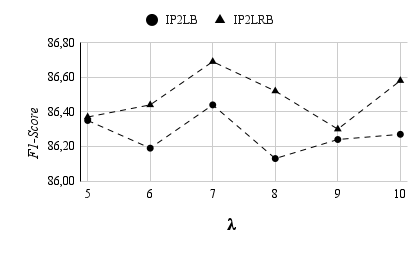
\includegraphics[width=\textwidth]{figures/f1-score-tau-1.png}
        \caption{Valores de \textit{F1-Score} dos métodos IP2LB e IP2LRB para $\tau=1$.}
        \label{fig:f1_score_tau_1}
    \end{subfigure}
    \begin{subfigure}[b]{0.49\textwidth}
        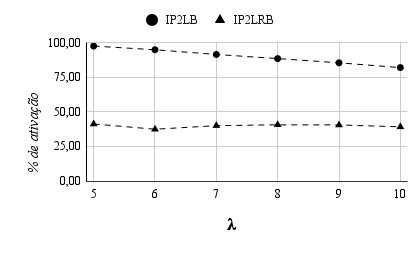
\includegraphics[width=\textwidth]{figures/binary-activation-tau-1.png}
        \caption{Percentual de ativação de busca binária dos métodos IP2LB e IP2LRB para $\tau=1$.}
        \label{fig:binary_activation_tau_1}
    \end{subfigure}
    \begin{subfigure}[b]{0.49\textwidth}
        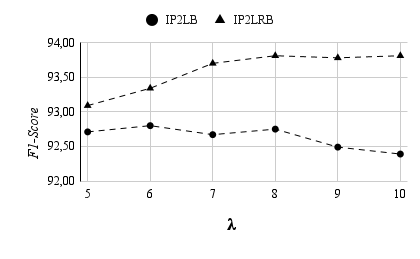
\includegraphics[width=\textwidth]{figures/f1-score-tau-2.png}
        \caption{Valores de \textit{F1-Score} dos métodos IP2LB e IP2LRB para $\tau=2$.}
        \label{fig:f1_score_tau_2}
    \end{subfigure}
    \begin{subfigure}[b]{0.49\textwidth}
        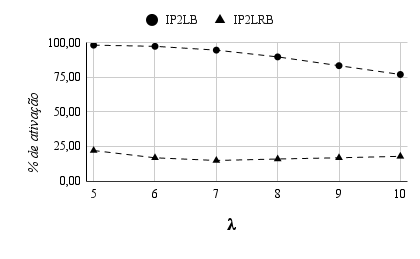
\includegraphics[width=\textwidth]{figures/binary-activation-tau-2.png}
        \caption{Percentual de ativação de busca binária dos métodos IP2LB e IP2LRB para $\tau=2$.}
        \label{fig:binary_activation_tau_2}
    \end{subfigure}
    \begin{subfigure}[b]{0.49\textwidth}
        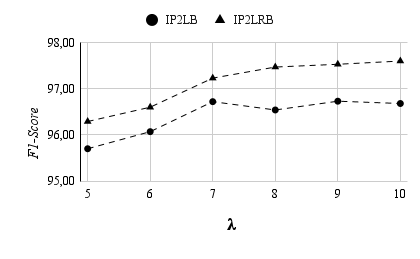
\includegraphics[width=\textwidth]{figures/f1-score-tau-3.png}
        \caption{Valores de \textit{F1-Score} dos métodos IP2LB e IP2LRB para $\tau=3$.}
        \label{fig:f1_score_tau_3}
    \end{subfigure}
    \begin{subfigure}[b]{0.49\textwidth}
        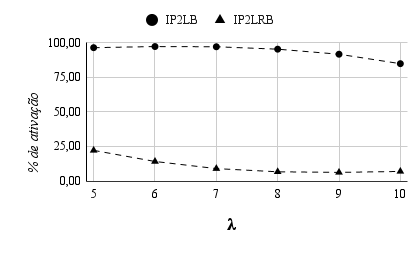
\includegraphics[width=\textwidth]{figures/binary-activation-tau-3.png}
        \caption{Percentual de ativação de busca binária dos métodos IP2LB e IP2LRB para $\tau=3$.}
        \label{fig:binary_activation_tau_3}
    \end{subfigure}
    \caption{Valores de \textit{F1-Score} e percentuais de ativação de busca binária para os métodos IP2LB e IP2LRB, com $\tau$ variando de $1$ a $3$ e $\lambda$ de $5$ a $10$, para a base JUSBRASIL.}
    \label{fig:f1_score_and_binary_activation}
\end{figure}


% Please add the following required packages to your document preamble:
% \usepackage{graphicx}
\begin{table}[h]
\centering
\resizebox{\textwidth}{!}{%
\begin{tabular}{c|cc|cc|cc|}
\cline{2-7}
\textbf{} & \multicolumn{2}{c|}{\textbf{$\tau=1$}} & \multicolumn{2}{c|}{\textbf{$\tau=2$}} & \multicolumn{2}{c|}{\textbf{$\tau=3$}} \\ \hline
\multicolumn{1}{|c|}{\textbf{Método}} & \textbf{\begin{tabular}[c|]{@{}c@{}}Tempo de \\ proc.\end{tabular}} & \textbf{F1-Score} & \textbf{\begin{tabular}[c]{@{}c@{}}Tempo de\\  proc.\end{tabular}} & \textbf{F1-Score} & \textbf{\begin{tabular}[c]{@{}c@{}}Tempo de\\  proc.\end{tabular}} & \textbf{F1-Score} \\ \hline
\multicolumn{1}{|c|}{IP2L-5} & 187,94 & 100,00 & 1906,07 & 100,00 & 15319,65 & 100,00 \\
\multicolumn{1}{|c|}{IP2LB-5} & 48,00 & 86,35 & 189,08 & 92,71 & 1642,66 & 95,70 \\
\multicolumn{1}{|c|}{IP2LRB-5} & 90,79 & 86,37 & 1170,75 & 93,09 & 8907,34 & 96,29 \\ \hline
\multicolumn{1}{|c|}{IP2L-6} & 97,93 & 100,00 & 792,27 & 100,00 & 8870,53 & 100,00 \\
\multicolumn{1}{|c|}{IP2LB-6} & 31,33 & 86,19 & 136,07 & 92,80 & 1145,92 & 96,07 \\
\multicolumn{1}{|c|}{IP2LRB-6} & 40,34 & 86,44 & 604,66 & 93,34 & 7339,66 & 96,60 \\ \hline
\multicolumn{1}{|c|}{IP2L-7} & 62,62 & 100,00 & 301,75 & 100,00 & 5607,94 & 100,00 \\
\multicolumn{1}{|c|}{IP2LB-7} & 17,86 & 86,44 & 76,48 & 92,67 & 720,42 & 96,72 \\
\multicolumn{1}{|c|}{IP2LRB-7} & 23,79 & 86,69 & 214,88 & 93,70 & 5112,13 & 97,23 \\ \hline
\multicolumn{1}{|c|}{IP2L-8} & 38,76 & 100,00 & 144,07 & 100,00 & 1905,70 & 100,00 \\
\multicolumn{1}{|c|}{IP2LB-8} & 12,78 & 86,13 & 49,68 & 92,75 & 328,13 & 96,54 \\
\multicolumn{1}{|c|}{IP2LRB-8} & 16,87 & 86,52 & 92,02 & 93,81 & 1778,79 & 97,47 \\ \hline
\multicolumn{1}{|c|}{IP2L-9} & 24,72 & 100,00 & 91,75 & 100,00 & 637,83 & 100,00 \\
\multicolumn{1}{|c|}{IP2LB-9} & 7,72 & 86,24 & 35,60 & 92,49 & 192,10 & 96,73 \\
\multicolumn{1}{|c|}{IP2LRB-9} & 10,75 & 86,30 & 64,30 & 93,78 & 567,71 & 97,53 \\ \hline
\multicolumn{1}{|c|}{IP2L-10} & 15,76 & 100,00 & 67,52 & 100,00 & 326,71 & 100,00 \\
\multicolumn{1}{|c|}{IP2LB-10} & 5,47 & 86,27 & 27,61 & 92,39 & 155,62 & 96,68 \\
\multicolumn{1}{|c|}{IP2LRB-10} & 7,70 & 86,58 & 49,50 & 93,81 & 279,60 & 97,60 \\ \hline
\multicolumn{1}{|c|}{BEVA} & 1,03 & 100,00 & 10,52 & 100,00 & 63,35 & 100,00 \\ \hline
\end{tabular}%
}
\caption{Tempo de processamento (ms) e F1-Score para os métodos IP2LB e IP2LRB e o método BEVA, variando o parâmetro $\lambda$ de $5$ a $10$ e $\tau$ de $1$ a $3$ na base de dados JUSBRASIL.}
\label{tab:f1-score-jusbrasil}
\end{table}

% Please add the following required packages to your document preamble:
% \usepackage{graphicx}
\begin{table}[]
\centering
\resizebox{\textwidth}{!}{%
\begin{tabular}{c|ccc|ccc|ccc|}
\cline{2-10}
\multicolumn{1}{l|}{\textbf{}} & \multicolumn{3}{c|}{\textbf{$\tau=1$}} & \multicolumn{3}{c|}{\textbf{$\tau=2$}} & \multicolumn{3}{c|}{\textbf{$\tau=3$}} \\ \hline
\multicolumn{1}{|c|}{\textbf{Método}} & \multicolumn{1}{c|}{\textbf{Nós Ativos}} & \multicolumn{1}{c|}{\textbf{\begin{tabular}[c]{@{}c@{}}Ativação \\ busca bin.\end{tabular}}} & \textbf{F1-Score} & \multicolumn{1}{c|}{\textbf{Nós Ativos}} & \multicolumn{1}{c|}{\textbf{\begin{tabular}[c]{@{}c@{}}Ativação \\ busca bin.\end{tabular}}} & \textbf{F1-Score} & \multicolumn{1}{c|}{\textbf{Nós Ativos}} & \multicolumn{1}{c|}{\textbf{\begin{tabular}[c]{@{}c@{}}Ativação \\ busca bin.\end{tabular}}} & \textbf{F1-Score} \\ \hline
\multicolumn{1}{|c|}{IP2LB-5} & 84,98 & 97,50\% & 86,35 & 2858,21 & 98,15\% & 92,71 & 26935,19 & 96,32\% & 95,70 \\
\multicolumn{1}{|c|}{IP2LRB-5} & 84,98 & 41,23\% & 86,37 & 2858,21 & 22,04\% & 93,09 & 26935,19 & 22,15\% & 96,29 \\ \hline
\multicolumn{1}{|c|}{IP2LB-6} & 59,18 & 94,82\% & 86,19 & 2064,35 & 97,30\% & 92,80 & 27976,40 & 97,14\% & 96,07 \\
\multicolumn{1}{|c|}{IP2LRB-6} & 59,18 & 37,42\% & 86,44 & 2064,35 & 16,79\% & 93,34 & 27976,40 & 14,14\% & 96,60 \\ \hline
\multicolumn{1}{|c|}{IP2LB-7} & 40,98 & 91,42\% & 86,44 & 1228,55 & 94,55\% & 92,67 & 23171,90 & 96,98\% & 96,72 \\
\multicolumn{1}{|c|}{IP2LRB-7} & 40,98 & 40,01\% & 86,69 & 1228,55 & 14,85\% & 93,70 & 23171,90 & 8,99\% & 97,23 \\ \hline
\multicolumn{1}{|c|}{IP2LB-8} & 32,78 & 88,44\% & 86,13 & 678,04 & 89,66\% & 92,75 & 15020,53 & 95,24\% & 96,54 \\
\multicolumn{1}{|c|}{IP2LRB-8} & 32,78 & 40,62\% & 86,52 & 678,04 & 15,92\% & 93,81 & 15020,53 & 6,69\% & 97,47 \\ \hline
\multicolumn{1}{|c|}{IP2LB-9} & 28,30 & 85,39\% & 86,24 & 428,66 & 83,32\% & 92,49 & 8289,18 & 91,59\% & 96,73 \\
\multicolumn{1}{|c|}{IP2LRB-9} & 28,30 & 40,51\% & 86,30 & 428,66 & 16,81\% & 93,78 & 8289,18 & 6,25\% & 97,53 \\ \hline
\multicolumn{1}{|c|}{IP2LB-10} & 24,84 & 81,94\% & 86,27 & 317,95 & 76,96\% & 92,39 & 4625,44 & 84,77\% & 96,68 \\
\multicolumn{1}{|c|}{IP2LRB-10} & 24,84 & 39,17\% & 86,58 & 317,95 & 17,86\% & 93,81 & 4625,44 & 6,95\% & 97,60 \\ \hline
\end{tabular}%
}
\caption{Média de nós ativos, percentual médio que indica em quanto dos nós ativos foi realizada a busca binária e F1-Score para os métodos IP2LB e IP2LRB, variando $\lambda$ de $5$ a $10$ e o $\tau$ de $1$ a $3$, na base JUSBRASIL.}
\label{tab:binary-search-activation}
\end{table}

Para $\tau=1$ os modelos IP2LB e IP2LRB obtiveram valores de \textit{F1-Score} muito próximos, apesar de baixos (menores do que $87\%$. O IP2LRB foi superficialmente mais preciso, como mostra a Figura~\ref{fig:f1_score_tau_1}. O IP2LB seguiu com os menores valores de tempo de processamento. Essa diferença de tempo de processamento ocorreu pois a busca binária foi utilizada em um grande percentual dos nós ativos no modelo IP2LB. Com $\lambda=5$, por exemplo, o IP2LB obteve $97,5\%$ de ativação da busca binária contra $41,23\%$ do IP2LRB, e com $\lambda=10$ o IP2LB obteve $81,94\%$ contra $39,17\%$ do IP2LRB, como mostra a Figura~\ref{fig:binary_activation_tau_1}. As linhas de tendência para \textit{F1-Score} não são muito claras para os dois métodos. 

Nas Figuras \ref{fig:binary_activation_tau_1}, \ref{fig:binary_activation_tau_2} e \ref{fig:binary_activation_tau_3} (as quais representam os dados das Tabelas \ref{tab:f1-score-jusbrasil} e \ref{tab:binary-search-activation}) nota-se que a curva de percentual de ativação segue um padrão decrescente para o modelo IP2LB, ou seja, à medida em que a quantidade de caracteres indexados na \textit{Trie} (valor de $\lambda$) aumenta, a busca binária ocorre em menos nós. Esse comportamento é esperado pois quanto maior o valor de $\lambda$, maior é a possibilidade de o primeiro nível do método ser o suficiente para conseguir responder à consulta utilizando nós ativos comuns, e não os nós de borda. 

Já o método IP2LRB apresenta um padrão de curva diferente. À medida em que $\lambda$ aumenta, o percentual de ativação começa a diminuir um pouco mas em seguida quase não apresenta mais diminuição. Isso provavelmente acontece devido à condição de restrição para ativação de busca binária que há no método. Quanto maior o valor de $\lambda$, mais raro é que surjam nós ativos de borda que foram ativados quando o $\lambda$-ésimo caractere foi processado pelo método. É provável que a maioria dos erros de digitação em um sistema de busca real como o da Jusbrasil ocorra nos primeiros caracteres da consulta, fazendo com que as sugestões sejam ativadas na \textit{Trie} antes de serem propagadas para o segundo nível.

Os dois modelos não se demonstraram muito vantajosos para $\tau=1$. Apesar de terem o tempo de processamento 2 ou até 3 vezes menores do que o IP2L para alguns valores de $\lambda$, os valores de \textit{F1-Score} parecem ser muito baixos quando se trata de um sistema real de CATE. Uma possível explicação para tais valores é que para $\tau=1$, a quantidade de nós ativos de borda é bem maior do que a quantidade de nós ativos comuns pois nesse caso os nós ativos comuns representam apenas correspondência sem erros de digitação (exata), então a busca binária será majoritariamente utilizada no segundo nível. Uma vez que ela é suscetível a recuperar algumas sugestões a mais, e também a ignorar outras sugestões que deveriam ser recuperadas, ativá-la com mais frequência pode causar diminuição significativa da acurácia.

Algo interessante a se notar é que enquanto os valores de \textit{F1-Score} foram próximos, há uma diferença considerável entre os percentuais de ativação de busca binária para os dois métodos. Um fato que pode ser extraído da definição dos dois métodos descritos na seção~\ref{sec:metodo} é que para um mesmo prefixo de consulta $p$ todo o conjunto de nós em que a busca binária foi ativada no método IP2LRB está completamente incluso no conjunto de nós de borda ativados no método IP2LB. 

A partir disso, uma possível explicação que surge é a de que os valores de \textit{F1-Score} do método IP2LRB definem um limite superior para os valores de \textit{F1-Score} do método IP2LB. É improvável que tal método ultrapasse os valores do IP2LRB pois realiza busca binária em um percentual de nós bem maior. Ao que tudo indica, o número maior de buscas binárias do IP2LB não impactou tanto a acurácia para $\tau=1$, e ajudou a reduzir o tempo de processamento em relação ao IP2LRB.

Para $\tau=2$, podemos ver com mais clareza o impacto do aumento da variável $\lambda$ nos valores de \textit{F1-Score}, além de os valores em si também estarem mais altos do que para $\tau=1$. Isso quer dizer que os dois métodos se apresentaram mais precisos quando passaram a tolerar mais um erro de digitação. Por outro lado o método IP2LB apresenta um padrão de diminuição gradual da métrica, e o IP2LRB apresenta uma linha de tendência logarítmica, que começa a estabilizar a partir de $\lambda=8$.

Há também uma maior disparidade entre os valores de \textit{F1-Score para os dois métodos}, chegando por exemplo a uma diferença de 1,42 para $\lambda=10$. Uma vez que a curva de ativação do método IP2LRB não apresenta muita variação à medida em que $\lambda$ cresce, e o valor de \textit{F1-Score} aumenta um pouco e depois estabiliza, é provável que haja um crescimento da quantidade de prefixos de consulta que são processados apenas no primeiro nível, o que explicaria o aumento da métrica. Como demonstrado na seção~\ref{sec:IP2LRB}, a busca binária introduz erro na recuperação das sugestões. Portanto, quanto menos ela é ativada, maior a acurácia, porém maior também é o tempo de processamento.

Com $\tau=3$, a linha de tendência para o método IP2LRB ainda permanece com características logarítmicas, mas agora o IP2LB também assume um formato próximo de linha tendência logarítmica (com exceção do ponto para $\lambda=8$). Além disso, há o ápice de \textit{F1-Score} para os dois métodos, chegando a $97,60\%$ para o IP2LRB com $\lambda=10$ e $96,73\%$ para o IP2LB com $\lambda=9$. Mais uma vez, verificamos que aumentar o valor de $\tau$ também aumentou a acurácia dos métodos. A hipótese para explicar esse fenômeno é que, devido à natureza exponencial do índice \textit{Trie} para o problema do CATE, e ao algoritmo ICPAN para computação de nós ativos, a quantidade de nós ativos de borda aumenta consideravelmente junto com o aumento de $\tau$; além disso, quanto mais erros são tolerados na busca no índice e mais profunda é a busca adiante nos níveis dos nós, menores são as chances de que eles contenham sugestões que respondam à consulta. Portanto, nesse caso a busca binária acaba auxiliando a não despender muito tempo processando esses nós.

Tal cenário de $\tau=3$ pode apresentar uma vantagem prática da combinação de busca binária e sequencial no segundo nível, estando relacionado à questão de pesquisa iii). O método IP2LB obteve um tempo de processamento 3 vezes menor do que o IP2L e quase 3 vezes menor também do que o IP2LRB para $\lambda=9$. Para $\lambda=10$ houve uma redução dos tempos de processamento dos métodos IP2L e IP2LRB, porém o IP2LB ainda permaneceu à frente, e apresentando uma boa acurácia. Na Tabela~\ref{tab:f1-score-jusbrasil} também há os tempos de processamento do método BEVA para $\tau$ variando de $1$ a $3$. O método desempenha muito bem para a base JUSBRASIL, obtendo média de tempo de processamento menor do que \textit{100ms} em cada valor de $\tau$. No entanto, como será demonstrado na seção~\ref{sec:memory_consumption}, o BEVA consome quase o triplo de memória do que qualquer um dos três métodos descritos na seção~\ref{sec:metodo}. 

Considerando o limite de 100ms para tempo de resposta \citep{ji2009efficient}, os métodos IP2L e IP2LRB demonstram-se lentos para $\tau=3$. O método IP2LB também ultrapassou essa marca em 55ms aproximadamente, apesar de ser o mais rápido dos métodos de nois níveis cenário. Os métodos IP2LB e IP2LRB nada mais são do que o método IP2L com a ativação da busca binária nos nós de borda, com diferentes critérios para ativá-la. 

Há espaço para a criação de um modelo que utiliza a estratégia do IP2L para $\tau \leq 2$, onde a acurácia é mais importante, e a do IP2LB para $\tau > 2$ onde mais importa a velocidade de resposta, já que o espaço amostral de sugestões de consultas que devem ser retornadas aumenta bastante. A diferença de \textit{F1-Score} entre o IP2LB e IP2LRB para $\tau=3$ foi inexpressiva, portanto faz sentido utilizar o IP2LB nesse possível novo modelo por conta de seu menor tempo de processamento. Nesse caso, seria possível atingir a marca de 100ms para $\tau \leq 3$ em bases um pouco menores do que a JUSBRASIL. Por fim, a questão de pesquisa i) pode ser empiricamente respondida pelos experimentos realizados, os quais demonstram que não é possível adaptar sistemas de busca em dois níveis para tirarem proveito da busca binária no segundo nível sem que haja algum impacto na acurácia do método.

\section{Avaliando os parâmetros dos métodos propostos}

Nessa seção iremos realizar a seleção do parâmetro $\lambda$ para os métodos IP2L, IP2LB e IP2LRB propostos na seção~\ref{sec:metodo}, com valores variando de $5$ a $10$. Não analisamos valores abaixo de $5$ pois o processamento da consulta ficaria custoso demais devido à frequente ativação do segundo nível. Semelhantemente, também não analisamos valores acima de $10$ pois grande parte do processamento da consulta ocorreria no primeiro nível. O objetivo dessa seção é estudar os efeitos de diferentes valores de $\lambda$ nos três métodos e escolher o melhor valor para os métodos considerando a acurácia, o tempo de processamento das consultas, e também consumo de memória.


\subsection{Tempo de processamento de prefixos de consulta}
\label{sec:methods-processing-time}

O tempo de processamento das consultas é uma métrica muito importante para avaliar sistemas de CATE. Essa métrica permite distinguir os algoritmos lentos dos rápidos para então escolher quais irão proporcionar a melhor experiência para o usuário, evitando atrasos notáveis e exibindo respostas a cada caractere digitado. Nós medimos o tempo de processamento em cada um dos dois níveis, portanto, o valor da coluna ``total'' nas tabelas dos experimentos é igual a soma dos valores das colunas ``1º'' e ``2º'' e representa o valor total do tempo de processamento. As Tabelas \ref{tab:methods-processing-time-tau-1-AOL} e  \ref{tab:methods-processing-time-tau-1-USADDR} contêm, considerando uma tolerância de $\tau=1$ erros de digitação, as medições dos tempos de processamento para os variados tamanhos de prefixos de consulta. Semelhantemente, as Tabelas \ref{tab:methods-processing-time-tau-2-AOL} e \ref{tab:methods-processing-time-tau-2-USADDR} para $\tau=2$ e as Tabelas \ref{tab:methods-processing-time-tau-3-AOL} e \ref{tab:methods-processing-time-tau-3-USADDR} para $\tau=3$.

Para facilitar a visualização dos dados contidos nas tabelas, também serão apresentadas figuras com um gráfico de barras empilhadas e agrupadas pelo valor de $\lambda$ variando de $5$ a $10$, para cada tamanho do prefixo de consulta. Em cada gráfico, para cada valor de $\lambda$ há um grupo de $3$ barras, uma para cada método proposto na seção~\ref{sec:metodo}. Cada barra é empilhada, contendo os tempos de processamento do primeiro nível (cor mais intensa) e segundo nível (cor mais clara). A altura final das barras empilhadas representa o tempo total de processamento do método.

\begin{figure} [h]
    \centering
    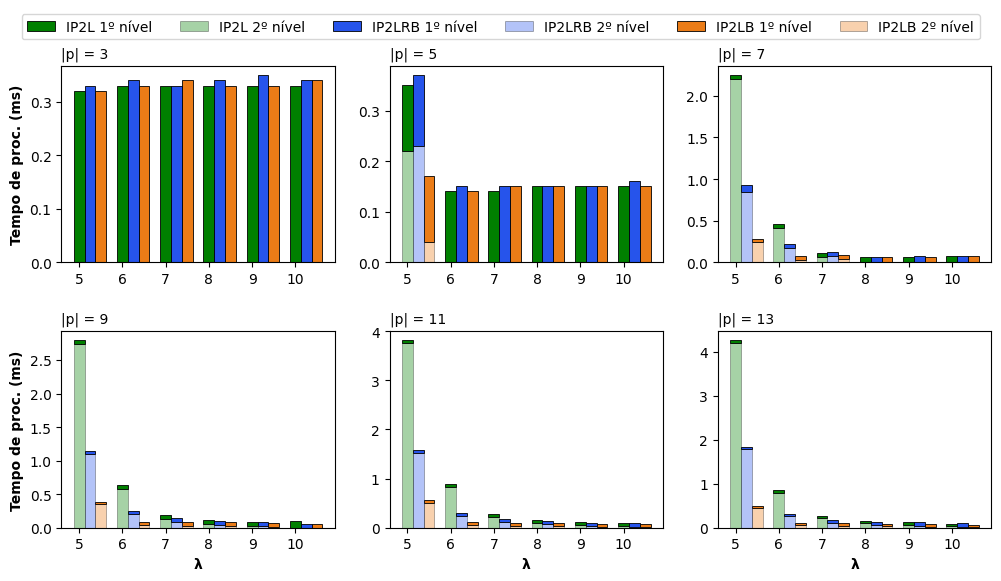
\includegraphics[width=1.0\textwidth]{figures/methods_processing_time_aol_1.png}
    \caption{Gráficos de barras empilhadas agrupadas por método (IP2L, IP2LB e IP2LRB) com o tempo de processamento (ms) em cada valor de $\lambda$ variando de $5$ a $10$, para $\tau=1$ e a base AOL.}
    \label{fig:methods_processing_time_aol_1}
\end{figure}

Para exemplificar, no primeiro gráfico para $|p|=3$ e base AOL da Figura~\ref{fig:methods_processing_time_aol_1} pode-se observar que há apenas barras com cores intensas, sem o empilhamento. Isso se deve ao fato de que o segundo nível não foi ativado em nenhum dos três métodos para $\tau=1$ e $\lambda=5$ pois a condição $|p| + \tau \leq \lambda$ ($3 + 1 \leq 5$) explicada na seção~\ref{sec:general_two_level_algorithm} foi satisfeita. Também é possível verificar na Tabela~\ref{tab:methods-processing-time-tau-1-AOL} a ausência de valores para a coluna  ``2º'' no grupo de $|p|=3$ junto às linhas dos métodos IP2L-5, IP2LB-5 e IP2LRB-5. À medida em que o tamanho de $p$ vai aumentando, também o segundo nível vai sendo ativado para maiores valores de $\lambda$.

Um padrão evidente e interessante que ocorre nos gráficos de $|p|=3$ e $|p|=5$ na Figura~\ref{fig:methods_processing_time_aol_1} é a semelhança de altura das barras quando somente o primeiro nível é ativado. Isso acontece porque o algoritmo do primeiro nível, o ICPAN, é compartilhado entre os três métodos, então essas barras representam simplesmente a média de tempo de processamento desse algoritmo para os devidos tamanhos de prefixo de consulta. É importante ressaltar que nas condições em que os métodos IP2L, IP2LB e IP2LRB foram apresentados na seção~\ref{sec:metodo}, qualquer um desses três métodos será equivalente ao ICPAN se $\lambda=\infty$. Nos 4 gráficos de barras seguintes da Figura~\ref{fig:methods_processing_time_aol_1} fica difícil notar esse mesmo padrão por conta do achatamento das barras devido aos altos tempos de processamento para $\lambda=5$, no entanto podemos observar na Tabela~\ref{tab:methods-processing-time-tau-1-AOL} que quando o segundo nível não é ativado em um valor de $\lambda$ qualquer, os valores de tempo total de processamento para os três métodos são estritamente próximos. Além disso, também é possível notar esse mesmo padrão para os valores de $\tau=2$ e $\tau=3$ na base AOL, e também para os valores de $\tau$ de $1$ a $3$ na base USADDR.

Para $|p|=5$ podemos observar o segundo nível sendo ativado quando $\lambda=5$. O tempo do primeiro nível permanece em torno de $0,14ms$ para os três métodos, mas a variação do tempo de processamento no segundo nível é quem determina boa parte do tempo de processamento final. No entanto, quanto maior o $\lambda$, menor é a influência do segundo nível no tempo de processamento final, chegando até mesmo a dividir valores semelhantes ao tempo do primeiro nível em alguns casos. Curiosamente o IP2LRB obteve um tempo ligeiramente maior no segundo nível em relação ao IP2L. Essa situação não acontece para valores maiores de $|p|$, porém se repete para as duas bases também com outros valores de $\tau$, como podemos observar nas Figuras \ref{fig:methods_processing_time_usaddr_1}, \ref{fig:methods_processing_time_aol_2}, \ref{fig:methods_processing_time_usaddr_2}, e \ref{fig:methods_processing_time_usaddr_3}. Uma possível explicação é a de que o percentual de ativação de busca binária não é tão alto para esses casos no método IP2LRB, então uma parte significativa do processamento do segundo nível acaba sendo a busca sequencial, a qual é mais dispendiosa, enquanto as buscas binárias são executadas com frequência na situação de pior caso. O IP2LB foi duas vezes mais rápido do que o IP2L, mas vale relembrar que para $\tau=1$ e $\tau=2$ a acurácia dos métodos IP2LB e IP2LRB pode deixar a desejar.


% Please add the following required packages to your document preamble:
% \usepackage{graphicx}
\begin{table}[h]
\centering
\resizebox{\textwidth}{!}{%
\begin{tabular}{c|ccc|ccc|ccc|ccc|ccc|ccc|}
\cline{2-19}
\multicolumn{1}{l|}{} &
  \multicolumn{3}{c|}{$|p|=3$} &
  \multicolumn{3}{c|}{$|p|=5$} &
  \multicolumn{3}{c|}{$|p|=7$} &
  \multicolumn{3}{c|}{$|p|=9$} &
  \multicolumn{3}{c|}{$|p|=11$} &
  \multicolumn{3}{c|}{$|p|=13$} \\ \hline
\multicolumn{1}{|c|}{\textbf{Método}} &
  \multicolumn{1}{c|}{\textbf{1º}} &
  \multicolumn{1}{c|}{\textbf{2º}} &
  \textbf{total} &
  \multicolumn{1}{c|}{\textbf{1º}} &
  \multicolumn{1}{c|}{\textbf{2º}} &
  \textbf{total} &
  \multicolumn{1}{c|}{\textbf{1º}} &
  \multicolumn{1}{c|}{\textbf{2º}} &
  \textbf{total} &
  \multicolumn{1}{c|}{\textbf{1º}} &
  \multicolumn{1}{c|}{\textbf{2º}} &
  \textbf{total} &
  \multicolumn{1}{c|}{\textbf{1º}} &
  \multicolumn{1}{c|}{\textbf{2º}} &
  \textbf{total} &
  \multicolumn{1}{c|}{\textbf{1º}} &
  \multicolumn{1}{c|}{\textbf{2º}} &
  \textbf{total} \\ \hline
\multicolumn{1}{|c|}{IP2L-5}    & 0,32 &  & 0,32 & 0,13 & 0,22 & 0,35 & 0,05 & 2,2  & 2,24 & 0,05 & 2,74 & 2,79 & 0,05 & 3,76 & 3,81 & 0,05 & 4,21 & 4,26 \\
\multicolumn{1}{|c|}{IP2LB-5}   & 0,32 &  & 0,32 & 0,13 & 0,04 & 0,17 & 0,04 & 0,24 & 0,28 & 0,04 & 0,35 & 0,39 & 0,05 & 0,51 & 0,56 & 0,05 & 0,45 & 0,50 \\
\multicolumn{1}{|c|}{IP2LRB-5}  & 0,33 &  & 0,33 & 0,14 & 0,23 & 0,36 & 0,08 & 0,85 & 0,94 & 0,05 & 1,1  & 1,15 & 0,06 & 1,52 & 1,58 & 0,06 & 1,78 & 1,84 \\ \hline
\multicolumn{1}{|c|}{IP2L-6}    & 0,33 &  & 0,33 & 0,14 &      & 0,14 & 0,05 & 0,41 & 0,46 & 0,05 & 0,58 & 0,63 & 0,05 & 0,83 & 0,89 & 0,05 & 0,8  & 0,85 \\
\multicolumn{1}{|c|}{IP2LB-6}   & 0,33 &  & 0,33 & 0,14 &      & 0,14 & 0,05 & 0,03 & 0,08 & 0,05 & 0,04 & 0,09 & 0,05 & 0,06 & 0,11 & 0,05 & 0,06 & 0,11 \\
\multicolumn{1}{|c|}{IP2LRB-6}  & 0,34 &  & 0,34 & 0,15 &      & 0,15 & 0,05 & 0,17 & 0,22 & 0,05 & 0,2  & 0,26 & 0,05 & 0,24 & 0,29 & 0,05 & 0,26 & 0,31 \\ \hline
\multicolumn{1}{|c|}{IP2L-7}    & 0,33 &  & 0,33 & 0,14 &      & 0,14 & 0,05 & 0,06 & 0,11 & 0,06 & 0,13 & 0,19 & 0,06 & 0,21 & 0,27 & 0,06 & 0,21 & 0,27 \\
\multicolumn{1}{|c|}{IP2LB-7}   & 0,34 &  & 0,34 & 0,15 &      & 0,15 & 0,05 & 0,04 & 0,09 & 0,05 & 0,03 & 0,08 & 0,06 & 0,04 & 0,10 & 0,06 & 0,04 & 0,09 \\
\multicolumn{1}{|c|}{IP2LRB-7}  & 0,33 &  & 0,33 & 0,15 &      & 0,15 & 0,05 & 0,07 & 0,12 & 0,06 & 0,08 & 0,14 & 0,06 & 0,12 & 0,18 & 0,06 & 0,11 & 0,17 \\ \hline
\multicolumn{1}{|c|}{IP2L-8}    & 0,33 &  & 0,33 & 0,15 &      & 0,15 & 0,06 &      & 0,06 & 0,06 & 0,05 & 0,11 & 0,06 & 0,1  & 0,16 & 0,06 & 0,1  & 0,16 \\
\multicolumn{1}{|c|}{IP2LB-8}   & 0,33 &  & 0,33 & 0,15 &      & 0,15 & 0,06 &      & 0,06 & 0,06 & 0,02 & 0,08 & 0,06 & 0,03 & 0,08 & 0,06 & 0,03 & 0,08 \\
\multicolumn{1}{|c|}{IP2LRB-8}  & 0,34 &  & 0,34 & 0,15 &      & 0,15 & 0,06 &      & 0,06 & 0,06 & 0,04 & 0,10 & 0,06 & 0,07 & 0,13 & 0,06 & 0,07 & 0,13 \\ \hline
\multicolumn{1}{|c|}{IP2L-9}    & 0,33 &  & 0,33 & 0,15 &      & 0,15 & 0,06 &      & 0,06 & 0,06 & 0,02 & 0,08 & 0,06 & 0,06 & 0,12 & 0,06 & 0,06 & 0,12 \\
\multicolumn{1}{|c|}{IP2LB-9}   & 0,33 &  & 0,33 & 0,15 &      & 0,15 & 0,06 &      & 0,06 & 0,06 & 0,01 & 0,07 & 0,06 & 0,02 & 0,08 & 0,06 & 0,02 & 0,08 \\
\multicolumn{1}{|c|}{IP2LRB-9}  & 0,35 &  & 0,35 & 0,15 &      & 0,15 & 0,08 &      & 0,08 & 0,06 & 0,02 & 0,08 & 0,06 & 0,04 & 0,10 & 0,08 & 0,04 & 0,12 \\ \hline
\multicolumn{1}{|c|}{IP2L-10}   & 0,33 &  & 0,33 & 0,15 &      & 0,15 & 0,07 &      & 0,07 & 0,10 &      & 0,10 & 0,06 & 0,03 & 0,09 & 0,06 & 0,03 & 0,10 \\
\multicolumn{1}{|c|}{IP2LB-10}  & 0,34 &  & 0,34 & 0,15 &      & 0,15 & 0,07 &      & 0,07 & 0,06 &      & 0,06 & 0,06 & 0,01 & 0,07 & 0,06 & 0,01 & 0,07 \\
\multicolumn{1}{|c|}{IP2LRB-10} & 0,34 &  & 0,34 & 0,16 &      & 0,16 & 0,07 &      & 0,07 & 0,06 &      & 0,06 & 0,07 & 0,02 & 0,09 & 0,08 & 0,02 & 0,10 \\ \hline
\end{tabular}%
}
\caption{Tempo de processamento (ms) dos métodos IP2L, IP2LB e IP2LRB para prefixos de consulta com tamanho $3,5,6,9,11$ e $13$, valores de $\lambda$ variando de $5$ a $10$, e para $\tau=1$ na base de dados AOL.}
\label{tab:methods-processing-time-tau-1-AOL}
\end{table}


\begin{figure} [h]
    \centering
    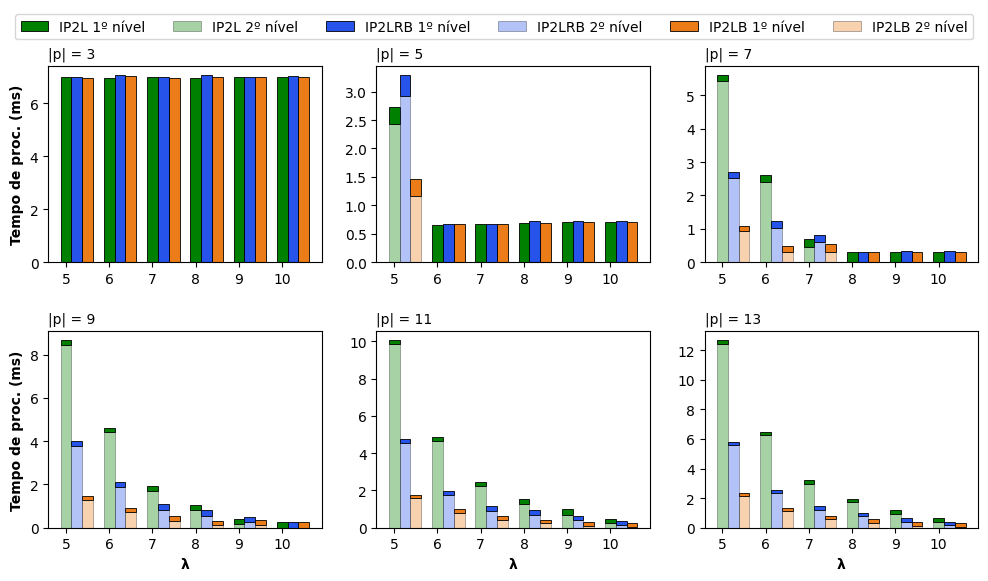
\includegraphics[width=1.0\textwidth]{figures/methods_processing_time_usaddr_1.png}
    \caption{Gráficos de barras empilhadas agrupadas por método (IP2L, IP2LB e IP2LRB) com o tempo de processamento (ms) em cada valor de $\lambda$ variando de $5$ a $10$, para $\tau=1$ e a base USADDR.}
    \label{fig:methods_processing_time_usaddr_1}
\end{figure}

% No entanto, vale ressaltar que as barras estão um pouco mais altas em comparação com a Figura~\ref{fig:methods_processing_time_aol_1}. Isso ocorre porque como há uma grande quantidade de itens na base, não só há mais nós indexados na \textit{Trie} como também o espaço amostral aumenta muito para a busca no segundo nível.

Na Figura~\ref{fig:methods_processing_time_usaddr_1} é possível observar a diferença de ordem de grandeza do eixo vertical de Tempo de Processamento em comparação com a Figura~\ref{fig:methods_processing_time_aol_1}, o que é esperado devido à magnitude de sugestões indexáveis da base USADDR. Todos os modelos em todos os valores de $\lambda$ conseguem manter a média de tempo de processamento bem distante de $100ms$ para todos os tamanhos de prefixo de consulta testados e $\tau=1$, mesmo para uma base maior como a USADDR. Também nota-se que os padrões de cada gráfico de barras da Figura~\ref{fig:methods_processing_time_usaddr_1} são muito similares aos padrões da Figura~\ref{fig:methods_processing_time_aol_1}. Isso demonstra que uma diferença expressiva no tamanho da base como há entre USADDR e AOL não desestabiliza os métodos nos diversos valores de $\lambda$. Se o tempo de processamento estiver alto demais devido ao tamanho de uma base, desde que haja memória suficiente sempre é possível experimentar aumentar o valor de $\lambda$ para encontrar um ponto de equilíbrio entre o desempenho e memória. Para $|p|=3$ os três métodos em todos os valores de $\lambda$ apresentaram tempo de processamento um pouco mais do que $6ms$, diminuindo bastante para valores maiores de $|p|$. Isso ocorre porque buscas por prefixos pequenos são muito custosas em sistemas de CATE, pois o conjunto de nós ativos fica muito populoso \citep{xiao2013efficient, berg2020}.

A eficiência do segundo nível do IP2LB devido à busca binária pode ser notada nos gráficos. A barra laranja de cor clara é menor do que as barras claras verde e azul na grande maioria dos casos, principalmente para valores menores de $\lambda$ como $5$ e $6$. Para os gráficos de $|p|=11$ e $|p|=13$ por exemplo, onde o segundo nível é ativado para todos os valores de $\lambda$, podemos observar que nos dois gráficos os tempos de processamento do método IP2LB começam bem mais abaixo do que os tempos dos outros dois métodos nos primeiros valores de $\lambda$. Tal padrão é comum em todos os gráficos de barras para $|p|=11$ e $|p|=13$ desta seção, ou seja, para as bases USADDR e AOL, e $\tau=1$ até $\tau=3$.

% Please add the following required packages to your document preamble:
% \usepackage{graphicx}
\begin{table}[h]
\centering
\resizebox{\textwidth}{!}{%
\begin{tabular}{c|ccc|ccc|ccc|ccc|ccc|ccc|}
\cline{2-19}
\multicolumn{1}{l|}{} &
  \multicolumn{3}{c|}{$|p|=3$} &
  \multicolumn{3}{c|}{$|p|=5$} &
  \multicolumn{3}{c|}{$|p|=7$} &
  \multicolumn{3}{c|}{$|p|=9$} &
  \multicolumn{3}{c|}{$|p|=11$} &
  \multicolumn{3}{c|}{$|p|=13$} \\ \hline
\multicolumn{1}{|c|}{\textbf{Método}} &
  \multicolumn{1}{c|}{\textbf{1º}} &
  \multicolumn{1}{c|}{\textbf{2º}} &
  \textbf{total} &
  \multicolumn{1}{c|}{\textbf{1º}} &
  \multicolumn{1}{c|}{\textbf{2º}} &
  \textbf{total} &
  \multicolumn{1}{c|}{\textbf{1º}} &
  \multicolumn{1}{c|}{\textbf{2º}} &
  \textbf{total} &
  \multicolumn{1}{c|}{\textbf{1º}} &
  \multicolumn{1}{c|}{\textbf{2º}} &
  \textbf{total} &
  \multicolumn{1}{c|}{\textbf{1º}} &
  \multicolumn{1}{c|}{\textbf{2º}} &
  \textbf{total} &
  \multicolumn{1}{c|}{\textbf{1º}} &
  \multicolumn{1}{c|}{\textbf{2º}} &
  \textbf{total} \\ \hline
\multicolumn{1}{|c|}{IP2L-5}    & 6,99 &  & 6,99 & 0,30 & 2,43 & 2,73 & 0,19 & 5,41 & 5,60 & 0,21 & 8,44 & 8,64 & 0,20 & 9,85 & 10,06 & 0,21 & 12,44 & 12,66 \\
\multicolumn{1}{|c|}{IP2LB-5}   & 6,96 &  & 6,96 & 0,30 & 1,16 & 1,45 & 0,17 & 0,93 & 1,10 & 0,18 & 1,3  & 1,47 & 0,18 & 1,59 & 1,77  & 0,20 & 2,14  & 2,34  \\
\multicolumn{1}{|c|}{IP2LRB-5}  & 7,00 &  & 7,00 & 0,36 & 2,93 & 3,29 & 0,18 & 2,52 & 2,70 & 0,25 & 3,76 & 4,01 & 0,21 & 4,55 & 4,75  & 0,22 & 5,59  & 5,81  \\ \hline
\multicolumn{1}{|c|}{IP2L-6}    & 6,96 &  & 6,96 & 0,66 &      & 0,66 & 0,20 & 2,4  & 2,60 & 0,21 & 4,42 & 4,63 & 0,21 & 4,66 & 4,87  & 0,22 & 6,25  & 6,47  \\
\multicolumn{1}{|c|}{IP2LB-6}   & 7,02 &  & 7,02 & 0,67 &      & 0,67 & 0,19 & 0,31 & 0,50 & 0,20 & 0,71 & 0,91 & 0,19 & 0,8  & 0,99  & 0,21 & 1,12  & 1,32  \\
\multicolumn{1}{|c|}{IP2LRB-6}  & 7,07 &  & 7,07 & 0,68 &      & 0,68 & 0,20 & 1,03 & 1,23 & 0,21 & 1,88 & 2,09 & 0,22 & 1,77 & 1,99  & 0,20 & 2,35  & 2,55  \\ \hline
\multicolumn{1}{|c|}{IP2L-7}    & 6,98 &  & 6,98 & 0,68 &      & 0,68 & 0,23 & 0,47 & 0,69 & 0,21 & 1,7  & 1,91 & 0,21 & 2,22 & 2,43  & 0,22 & 2,98  & 3,20  \\
\multicolumn{1}{|c|}{IP2LB-7}   & 6,96 &  & 6,96 & 0,68 &      & 0,68 & 0,23 & 0,31 & 0,54 & 0,20 & 0,32 & 0,52 & 0,20 & 0,44 & 0,64  & 0,23 & 0,58  & 0,80  \\
\multicolumn{1}{|c|}{IP2LRB-7}  & 7,01 &  & 7,01 & 0,68 &      & 0,68 & 0,22 & 0,61 & 0,84 & 0,26 & 0,84 & 1,10 & 0,23 & 0,92 & 1,15  & 0,21 & 1,23  & 1,45  \\ \hline
\multicolumn{1}{|c|}{IP2L-8}    & 6,96 &  & 6,96 & 0,69 &      & 0,69 & 0,31 &      & 0,31 & 0,22 & 0,82 & 1,04 & 0,23 & 1,3  & 1,53  & 0,23 & 1,74  & 1,97  \\
\multicolumn{1}{|c|}{IP2LB-8}   & 7,00 &  & 7,00 & 0,69 &      & 0,69 & 0,32 &      & 0,32 & 0,21 & 0,12 & 0,34 & 0,21 & 0,23 & 0,44  & 0,23 & 0,33  & 0,56  \\
\multicolumn{1}{|c|}{IP2LRB-8}  & 7,06 &  & 7,06 & 0,72 &      & 0,72 & 0,31 &      & 0,31 & 0,29 & 0,53 & 0,81 & 0,27 & 0,69 & 0,96  & 0,22 & 0,78  & 1,00  \\ \hline
\multicolumn{1}{|c|}{IP2L-9}    & 6,98 &  & 6,98 & 0,70 &      & 0,70 & 0,32 &      & 0,32 & 0,23 & 0,19 & 0,43 & 0,34 & 0,68 & 1,03  & 0,24 & 0,93  & 1,17  \\
\multicolumn{1}{|c|}{IP2LB-9}   & 7,00 &  & 7,00 & 0,70 &      & 0,70 & 0,31 &      & 0,31 & 0,24 & 0,12 & 0,36 & 0,23 & 0,1  & 0,33  & 0,25 & 0,15  & 0,40  \\
\multicolumn{1}{|c|}{IP2LRB-9}  & 7,00 &  & 7,00 & 0,73 &      & 0,73 & 0,34 &      & 0,34 & 0,26 & 0,25 & 0,51 & 0,24 & 0,39 & 0,63  & 0,23 & 0,42  & 0,65  \\ \hline
\multicolumn{1}{|c|}{IP2L-10}   & 7,00 &  & 7,00 & 0,70 &      & 0,70 & 0,31 &      & 0,31 & 0,27 &      & 0,27 & 0,24 & 0,23 & 0,47  & 0,24 & 0,4   & 0,64  \\
\multicolumn{1}{|c|}{IP2LB-10}  & 6,98 &  & 6,98 & 0,70 &      & 0,70 & 0,32 &      & 0,32 & 0,27 &      & 0,27 & 0,23 & 0,03 & 0,26  & 0,25 & 0,05  & 0,31  \\
\multicolumn{1}{|c|}{IP2LRB-10} & 7,04 &  & 7,04 & 0,72 &      & 0,72 & 0,35 &      & 0,35 & 0,26 &      & 0,26 & 0,24 & 0,13 & 0,38  & 0,23 & 0,18  & 0,41  \\ \hline
\end{tabular}%
}
\caption{Tempo de processamento (ms) dos métodos IP2L, IP2LB e IP2LRB para prefixos de consulta com tamanho $3,5,6,9,11$ e $13$, valores de $\lambda$ variando de $5$ a $10$, e para $\tau=1$ na base de dados USADDR.}
\label{tab:methods-processing-time-tau-1-USADDR}
\end{table}


\begin{figure} [h]
    \centering
    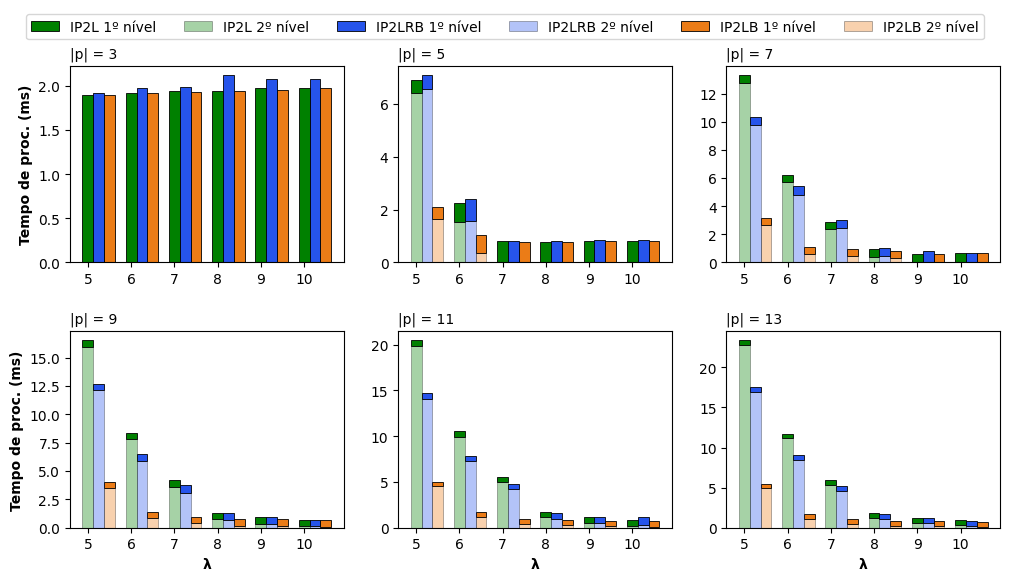
\includegraphics[width=1.0\textwidth]{figures/methods_processing_time_aol_2.png}
    \caption{Gráficos de barras empilhadas agrupadas por método (IP2L, IP2LB e IP2LRB) com o tempo de processamento (ms) em cada valor de $\lambda$ variando de $5$ a $10$, para $\tau=2$ e a base AOL.}
    \label{fig:methods_processing_time_aol_2}
\end{figure}

Para $\tau=2$ houve um aumento em geral na ordem de grandeza da média de tempo de processamento para valores mais baixos de $\lambda$ como 5 e 6 para o IP2L, tanto para AOL quanto para USADDR, na qual tal aumento é ainda mais evidente. Na Tabela~\ref{tab:methods-processing-time-tau-1-USADDR} temos por exemplo o IP2L-10 com $0,47ms$ para $|p|=11$ contra $7,05ms$ para o mesmo método e tamanho de $p$ na Tabela~\ref{tab:methods-processing-time-tau-2-USADDR}. O aumento no valor de $\tau$ faz com que o conjunto de nós ativos do primeiro nível cresça bastante, e como consequência a quantidade de itens para serem buscados sequencialmente também aumenta no segundo nível. No entanto, os métodos seguem tendo uma boa média de tempo para $\lambda=10$. Podemos verificar na Tabela~\ref{tab:methods-processing-time-tau-2-AOL} para $|p|=13$ por exemplo que o IP2L-10 foi cerca de 25 vezes mais rápido do que o IP2L-5, mas apesar disso o método IP2LB-10 foi somente 7 vezes mais rápido que o IP2LB-5. Comparando somente o tempo no segundo nível ainda para $|p|=13$, por exemplo, temos que o segundo nível do IP2L-10 foi cerca de 81 vezes mais rápido que o do IP2L-5. Considerando que há pouca variação entre os tempos do primeiro nível à medida em que $|p|$ vai aumentando, um valor maior de $\lambda$ de fato beneficia o segundo nível, pois o filtro do primeiro nível fica muito mais preciso.

Com a mudança do valor de $\tau$ o critério de ativação do segundo nível também mudou, por isso os gráficos da Figura~\ref{fig:methods_processing_time_aol_2} e \ref{fig:methods_processing_time_usaddr_2} possuem padrões diferentes nas sequências de grupos de barras. Para $|p|=5$ por exemplo o segundo nível agora é ativado para $\lambda=6$, pois $|p| + \tau > \lambda$ ($5 + 2 > 6$). Além disso, os tempos do IP2LRB ficaram mais relativamente próximos dos tempos do IP2L quando $\tau=2$ tanto para a base AOL quanto para USADDR. Isso talvez tenha acontecido porque o aumento de $\tau$ causou uma multiplicação significativa de nós ativos no segundo nível, mas o percentual de ativação da busca binária foi bem baixo (o que é esperado para o IP2LRB em alguns casos, devido à sua condição de restrição de ativação). 

% Please add the following required packages to your document preamble:
% \usepackage{graphicx}
\begin{table}[h]
\centering
\resizebox{\textwidth}{!}{%
\begin{tabular}{c|ccc|ccc|ccc|ccc|ccc|ccc|}
\cline{2-19}
\multicolumn{1}{l|}{} &
  \multicolumn{3}{c|}{$|p|=3$} &
  \multicolumn{3}{c|}{$|p|=5$} &
  \multicolumn{3}{c|}{$|p|=7$} &
  \multicolumn{3}{c|}{$|p|=9$} &
  \multicolumn{3}{c|}{$|p|=11$} &
  \multicolumn{3}{c|}{$|p|=13$} \\ \hline
\multicolumn{1}{|c|}{\textbf{Método}} &
  \multicolumn{1}{c|}{\textbf{1º}} &
  \multicolumn{1}{c|}{\textbf{2º}} &
  \textbf{total} &
  \multicolumn{1}{c|}{\textbf{1º}} &
  \multicolumn{1}{c|}{\textbf{2º}} &
  \textbf{total} &
  \multicolumn{1}{c|}{\textbf{1º}} &
  \multicolumn{1}{c|}{\textbf{2º}} &
  \textbf{total} &
  \multicolumn{1}{c|}{\textbf{1º}} &
  \multicolumn{1}{c|}{\textbf{2º}} &
  \textbf{total} &
  \multicolumn{1}{c|}{\textbf{1º}} &
  \multicolumn{1}{c|}{\textbf{2º}} &
  \textbf{total} &
  \multicolumn{1}{c|}{\textbf{1º}} &
  \multicolumn{1}{c|}{\textbf{2º}} &
  \textbf{total} \\ \hline
\multicolumn{1}{|c|}{IP2L-5}    & 1,89 &  & 1,89 & 0,49 & 6,4  & 6,89 & 0,53 & 12,78 & 13,32 & 0,54 & 15,96 & 16,50 & 0,56 & 19,89 & 20,44 & 0,56 & 22,8  & 23,37 \\
\multicolumn{1}{|c|}{IP2LB-5}   & 1,89 &  & 1,89 & 0,46 & 1,64 & 2,10 & 0,50 & 2,64  & 3,14  & 0,51 & 3,53  & 4,03  & 0,52 & 4,51  & 5,03  & 0,54 & 4,9   & 5,44  \\
\multicolumn{1}{|c|}{IP2LRB-5}  & 1,92 &  & 1,92 & 0,53 & 6,56 & 7,09 & 0,56 & 9,75  & 10,31 & 0,58 & 12,11 & 12,68 & 0,59 & 14,11 & 14,71 & 0,67 & 16,91 & 17,58 \\ \hline
\multicolumn{1}{|c|}{IP2L-6}    & 1,92 &  & 1,92 & 0,70 & 1,54 & 2,24 & 0,52 & 5,68  & 6,21  & 0,53 & 7,81  & 8,34  & 0,57 & 9,95  & 10,52 & 0,56 & 11,15 & 11,70 \\
\multicolumn{1}{|c|}{IP2LB-6}   & 1,92 &  & 1,92 & 0,70 & 0,34 & 1,04 & 0,51 & 0,56  & 1,07  & 0,52 & 0,86  & 1,39  & 0,53 & 1,15  & 1,68  & 0,53 & 1,15  & 1,67  \\
\multicolumn{1}{|c|}{IP2LRB-6}  & 1,97 &  & 1,97 & 0,80 & 1,58 & 2,37 & 0,66 & 4,78  & 5,44  & 0,57 & 5,92  & 6,49  & 0,59 & 7,25  & 7,84  & 0,70 & 8,41  & 9,11  \\ \hline
\multicolumn{1}{|c|}{IP2L-7}    & 1,94 &  & 1,94 & 0,79 &      & 0,79 & 0,55 & 2,35  & 2,90  & 0,56 & 3,62  & 4,18  & 0,59 & 4,95  & 5,54  & 0,58 & 5,33  & 5,91  \\
\multicolumn{1}{|c|}{IP2LB-7}   & 1,93 &  & 1,93 & 0,76 &      & 0,76 & 0,54 & 0,44  & 0,98  & 0,53 & 0,38  & 0,91  & 0,56 & 0,44  & 1,01  & 0,56 & 0,47  & 1,03  \\
\multicolumn{1}{|c|}{IP2LRB-7}  & 1,98 &  & 1,98 & 0,81 &      & 0,81 & 0,56 & 2,46  & 3,02  & 0,64 & 3,09  & 3,73  & 0,63 & 4,18  & 4,81  & 0,65 & 4,58  & 5,23  \\ \hline
\multicolumn{1}{|c|}{IP2L-8}    & 1,94 &  & 1,94 & 0,77 &      & 0,77 & 0,56 & 0,41  & 0,97  & 0,56 & 0,76  & 1,33  & 0,61 & 1,13  & 1,74  & 0,60 & 1,26  & 1,86  \\
\multicolumn{1}{|c|}{IP2LB-8}   & 1,94 &  & 1,94 & 0,78 &      & 0,78 & 0,55 & 0,28  & 0,83  & 0,57 & 0,19  & 0,76  & 0,58 & 0,25  & 0,84  & 0,59 & 0,26  & 0,85  \\
\multicolumn{1}{|c|}{IP2LRB-8}  & 2,12 &  & 2,12 & 0,82 &      & 0,82 & 0,58 & 0,43  & 1,00  & 0,61 & 0,71  & 1,33  & 0,65 & 0,97  & 1,62  & 0,65 & 1,09  & 1,74  \\ \hline
\multicolumn{1}{|c|}{IP2L-9}    & 1,97 &  & 1,97 & 0,80 &      & 0,80 & 0,61 &       & 0,61  & 0,58 & 0,34  & 0,92  & 0,63 & 0,53  & 1,16  & 0,62 & 0,6   & 1,21  \\
\multicolumn{1}{|c|}{IP2LB-9}   & 1,95 &  & 1,95 & 0,79 &      & 0,79 & 0,61 &       & 0,61  & 0,60 & 0,14  & 0,74  & 0,61 & 0,16  & 0,78  & 0,61 & 0,17  & 0,78  \\
\multicolumn{1}{|c|}{IP2LRB-9}  & 2,07 &  & 2,07 & 0,85 &      & 0,85 & 0,82 &       & 0,82  & 0,61 & 0,36  & 0,98  & 0,68 & 0,5   & 1,17  & 0,62 & 0,54  & 1,15  \\ \hline
\multicolumn{1}{|c|}{IP2L-10}   & 1,97 &  & 1,97 & 0,80 &      & 0,80 & 0,65 &       & 0,65  & 0,60 & 0,12  & 0,71  & 0,63 & 0,24  & 0,87  & 0,64 & 0,28  & 0,92  \\
\multicolumn{1}{|c|}{IP2LB-10}  & 1,97 &  & 1,97 & 0,81 &      & 0,81 & 0,64 &       & 0,64  & 0,59 & 0,07  & 0,65  & 0,63 & 0,08  & 0,71  & 0,63 & 0,09  & 0,72  \\
\multicolumn{1}{|c|}{IP2LRB-10} & 2,08 &  & 2,08 & 0,86 &      & 0,86 & 0,67 &       & 0,67  & 0,60 & 0,12  & 0,71  & 0,92 & 0,27  & 1,19  & 0,65 & 0,25  & 0,90  \\ \hline
\end{tabular}%
}
\caption{Tempo de processamento (ms) dos métodos IP2L, IP2LB e IP2LRB para prefixos de consulta com tamanho $3,5,6,9,11$ e $13$, valores de $\lambda$ variando de $5$ a $10$, e para $\tau=2$ na base de dados AOL.}
\label{tab:methods-processing-time-tau-2-AOL}
\end{table}


\begin{figure} [h]
    \centering
    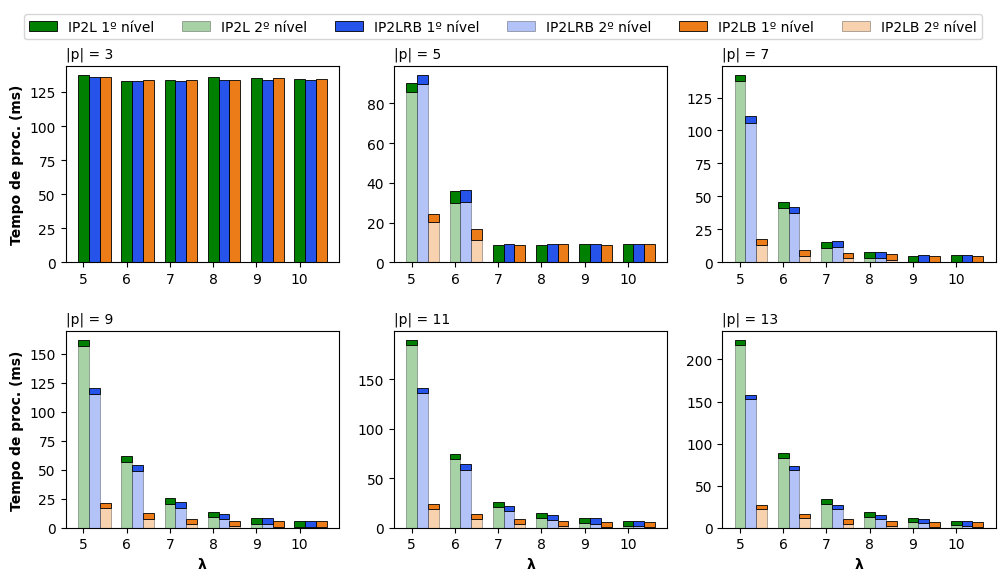
\includegraphics[width=1.0\textwidth]{figures/methods_processing_time_usaddr_2.png}
    \caption{Gráficos de barras empilhadas agrupadas por método (IP2L, IP2LB e IP2LRB) com o tempo de processamento (ms) em cada valor de $\lambda$ variando de $5$ a $10$, para $\tau=2$ e a base USADDR.}
    \label{fig:methods_processing_time_usaddr_2}
\end{figure}

Podemos observar através da Tabela~\ref{tab:methods-processing-time-tau-2-USADDR} que o modelo IP2L-5  dificilmente poderia ser utilizado em um sistema real com base tão grande quanto a USADDR. O único caso em que há média de tempo abaixo de $100ms$ é para $|p|=5$ e isso quando $\tau$ ainda é igual a 2. Já o modelo IP2L-10 possui média igual a $8,12ms$ para $|p|=13$, por exemplo. Essas evidências reforçam a ideia de que deve ser considerado um fator de proporcionalidade entre o valor de $\lambda$ e o tamanho da base de sugestões que será indexada, visando um equilíbrio entre a quantidade de memória utilizada e o tempo de processamento.

É importante ressaltar que os três métodos atingiram tempo maior que $100ms$ para $|p|=3$ na base USADDR, como indica claramente o primeiro gráfico da Figura~\ref{fig:methods_processing_time_usaddr_2}. Essa situação pode ser problemática em um sistema real de CATE com base de tamanho similar à USADDR. Considerando $|p|=3$, observamos nas Tabelas \ref{tab:methods-processing-time-tau-1-USADDR} e \ref{tab:methods-processing-time-tau-2-USADDR} que o aumento de $\tau=1$ para $\tau=2$ levou uma média de tempo de processamento dos métodos de $7ms$ para $134ms$. Nesse cenário não se pode esperar bons resultados para $\tau=3$. Essa expectativa negativa é confirmada no primeiro gráfico da Figura~\ref{fig:methods_processing_time_usaddr_1}. No entanto, para amenizar esse problema uma opção é utilizar uma técnica de \textit{cache} para manter conjuntos de nós pré-ativados para consultas pequenas de tamanho menor ou igual a 3, por exemplo. Esse tipo de técnica de \textit{cache} está presente na implementação do BEVA utilizada nesta pesquisa, e comprovadamente provoca grande diminuição no tempo de processamento para prefixos de consulta pequenos como $|p| \leq 3$, como veremos adiante na seção~\ref{sec:comparison_baseline_methods}.




% Please add the following required packages to your document preamble:
% \usepackage{graphicx}
\begin{table}[h]
\centering
\resizebox{\textwidth}{!}{%
\begin{tabular}{c|ccc|ccc|ccc|ccc|ccc|ccc|}
\cline{2-19}
\multicolumn{1}{l|}{} & \multicolumn{3}{c|}{$|p|=3$} & \multicolumn{3}{c|}{$|p|=5$} & \multicolumn{3}{c|}{$|p|=7$} & \multicolumn{3}{c|}{$|p|=9$} & \multicolumn{3}{c|}{$|p|=11$} & \multicolumn{3}{c|}{$|p|=13$} \\ \hline
\multicolumn{1}{|c|}{\textbf{Método}} & \multicolumn{1}{c|}{\textbf{1º}} & \multicolumn{1}{c|}{\textbf{2º}} & \textbf{total} & \multicolumn{1}{c|}{\textbf{1º}} & \multicolumn{1}{c|}{\textbf{2º}} & \textbf{total} & \multicolumn{1}{c|}{\textbf{1º}} & \multicolumn{1}{c|}{\textbf{2º}} & \textbf{total} & \multicolumn{1}{c|}{\textbf{1º}} & \multicolumn{1}{c|}{\textbf{2º}} & \textbf{total} & \multicolumn{1}{c|}{\textbf{1º}} & \multicolumn{1}{c|}{\textbf{2º}} & \textbf{total} & \multicolumn{1}{c|}{\textbf{1º}} & \multicolumn{1}{c|}{\textbf{2º}} & \textbf{total} \\ \hline
\multicolumn{1}{|c|}{IP2L-5} & 137,40 &  & 137,40 & 4,15 & 85,93 & 90,08 & 4,39 & 137,62 & 142,02 & 4,78 & 156,54 & 161,32 & 5,00 & 184,45 & 189,45 & 5,02 & 217,55 & 222,57 \\
\multicolumn{1}{|c|}{IP2LB-5} & 135,80 &  & 135,80 & 4,11 & 20,16 & 24,27 & 4,04 & 13,49 & 17,52 & 4,34 & 17,11 & 21,45 & 4,38 & 19,24 & 23,62 & 4,73 & 21,69 & 26,42 \\
\multicolumn{1}{|c|}{IP2LRB-5} & 136,31 &  & 136,31 & 4,36 & 89,91 & 94,27 & 4,89 & 105,91 & 110,81 & 4,90 & 115,56 & 120,46 & 5,14 & 136,14 & 141,28 & 5,09 & 152,69 & 157,78 \\ \hline
\multicolumn{1}{|c|}{IP2L-6} & 133,11 &  & 133,11 & 5,93 & 29,82 & 35,76 & 4,63 & 41,2 & 45,83 & 5,02 & 56,85 & 61,87 & 5,16 & 69,2 & 74,36 & 5,42 & 83,32 & 88,74 \\
\multicolumn{1}{|c|}{IP2LB-6} & 133,65 &  & 133,65 & 5,82 & 11,11 & 16,93 & 4,28 & 5,16 & 9,44 & 4,62 & 7,64 & 12,26 & 4,74 & 9,2 & 13,93 & 5,03 & 11,48 & 16,50 \\
\multicolumn{1}{|c|}{IP2LRB-6} & 133,36 &  & 133,36 & 5,96 & 30,36 & 36,32 & 4,74 & 37,07 & 41,82 & 5,27 & 48,9 & 54,16 & 5,31 & 58,76 & 64,07 & 5,32 & 68,33 & 73,65 \\ \hline
\multicolumn{1}{|c|}{IP2L-7} & 133,90 &  & 133,90 & 8,66 &  & 8,66 & 4,45 & 10,93 & 15,38 & 4,93 & 20,44 & 25,37 & 4,96 & 21,4 & 26,36 & 5,20 & 28,4 & 33,60 \\
\multicolumn{1}{|c|}{IP2LB-7} & 133,71 &  & 133,71 & 8,91 &  & 8,91 & 4,39 & 3,04 & 7,43 & 4,65 & 3,09 & 7,74 & 4,84 & 3,89 & 8,74 & 5,12 & 4,84 & 9,96 \\
\multicolumn{1}{|c|}{IP2LRB-7} & 133,32 &  & 133,32 & 9,11 &  & 9,11 & 4,40 & 11,47 & 15,88 & 5,11 & 16,85 & 21,97 & 5,15 & 17,2 & 22,35 & 5,21 & 22,22 & 27,43 \\ \hline
\multicolumn{1}{|c|}{IP2L-8} & 136,30 &  & 136,30 & 8,82 &  & 8,82 & 4,53 & 3,09 & 7,62 & 4,83 & 8,88 & 13,71 & 4,99 & 9,91 & 14,90 & 5,12 & 13,24 & 18,36 \\
\multicolumn{1}{|c|}{IP2LB-8} & 133,62 &  & 133,62 & 9,04 &  & 9,04 & 4,49 & 1,56 & 6,05 & 4,67 & 1,25 & 5,92 & 4,92 & 1,89 & 6,80 & 5,30 & 2,54 & 7,84 \\
\multicolumn{1}{|c|}{IP2LRB-8} & 133,62 &  & 133,62 & 9,28 &  & 9,28 & 4,63 & 3,15 & 7,77 & 4,83 & 7,24 & 12,08 & 5,26 & 7,74 & 13,00 & 5,19 & 10,12 & 15,31 \\ \hline
\multicolumn{1}{|c|}{IP2L-9} & 135,12 &  & 135,12 & 9,02 &  & 9,02 & 4,95 &  & 4,95 & 4,91 & 3,05 & 7,96 & 5,01 & 4,54 & 9,55 & 5,21 & 6,45 & 11,66 \\
\multicolumn{1}{|c|}{IP2LB-9} & 135,07 &  & 135,07 & 8,95 &  & 8,95 & 4,94 &  & 4,94 & 4,85 & 0,96 & 5,80 & 5,03 & 0,93 & 5,97 & 5,44 & 1,39 & 6,83 \\
\multicolumn{1}{|c|}{IP2LRB-9} & 133,89 &  & 133,89 & 9,34 &  & 9,34 & 5,28 &  & 5,28 & 5,08 & 3,28 & 8,36 & 5,66 & 3,88 & 9,54 & 5,26 & 5,09 & 10,35 \\ \hline
\multicolumn{1}{|c|}{IP2L-10} & 134,59 &  & 134,59 & 9,24 &  & 9,24 & 5,22 &  & 5,22 & 5,04 & 0,79 & 5,83 & 5,14 & 1,91 & 7,05 & 5,31 & 2,81 & 8,12 \\
\multicolumn{1}{|c|}{IP2LB-10} & 134,60 &  & 134,60 & 9,31 &  & 9,31 & 5,08 &  & 5,08 & 4,99 & 0,54 & 5,54 & 5,08 & 0,45 & 5,53 & 5,59 & 0,69 & 6,28 \\
\multicolumn{1}{|c|}{IP2LRB-10} & 133,78 &  & 133,78 & 9,26 &  & 9,26 & 5,44 &  & 5,44 & 4,96 & 0,81 & 5,76 & 5,42 & 1,65 & 7,07 & 5,44 & 2,19 & 7,64 \\ \hline
\end{tabular}%
}
\caption{Tempo de processamento (ms) dos métodos IP2L, IP2LB e IP2LRB para prefixos de consulta com tamanho $3,5,6,9,11$ e $13$, valores de $\lambda$ variando de $5$ a $10$, e para $\tau=2$ na base de dados USADDR.}
\label{tab:methods-processing-time-tau-2-USADDR}
\end{table}

\begin{figure} [h]
    \centering
    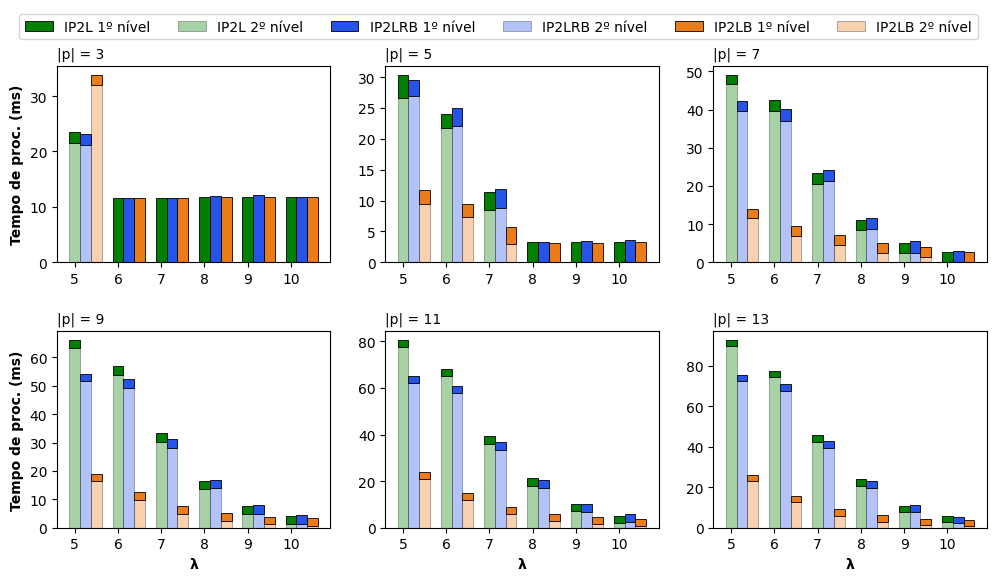
\includegraphics[width=1.0\textwidth]{figures/methods_processing_time_aol_3.png}
    \caption{Gráficos de barras empilhadas agrupadas por método (IP2L, IP2LB e IP2LRB) com o tempo de processamento (ms) em cada valor de $\lambda$ variando de $5$ a $10$, para $\tau=3$ e a base AOL.}
    \label{fig:methods_processing_time_aol_3}
\end{figure}

Para $\tau=3$ ocorre uma ``anomalia'' no gráfico de $|p|=3$ tanto para a base AOL quanto para USADDR. Uma vez que $|p| + \tau > \lambda$ ($3 + 3 > 5$) o segundo nível é ativado, e nesse caso a média de tempo de processamento IP2LB se mostrou maior que a dos outros dois métodos. No método IP2LB a busca binária é ativada em grande parte dos nós ativos, tendo muita participação no tempo total de execução do segundo nível, então é plausível considerar que essa diferença acontece possivelmente devido à busca binária estar se aproximando com frequência do pior caso, e também estar sendo realizada em listas muito grandes. Além disso, na base USADDR os três métodos não tiveram um bom desempenho para $|p|=3$ em nenhum valor de $\lambda$, com tempos de processamento maiores do que $500ms$. Os métodos originais ICAN e ICPAN também sofrem com esse problema, como veremos mais adiante na seção~\ref{sec:comparison_baseline_methods}. Como mencionado anteriormente essa situação pode ser mitigada ao utilizar estratégias de \textit{cache} de nós ativos.

Na base AOL os tempos de processamento para $\lambda=5$ com tamanhos de prefixos $|p|=11$ e $|p|=13$ já começam a se aproximar de $100ms$ nos modelos IP2L e IP2LRB. No entanto, vale ressaltar que o IP2L-5 por exemplo utiliza duas vezes menos memória do que o IP2L nessa base. Se um sistema real de CATE com base de sugestões de tamanho similar à AOL receber poucas consultas com tamanho maior do que 13 caracteres (o que é bem provável pois consultas longas são menos frequentes nesses sistemas), vale a pena considerar utilizar o IP2L-5 ou IP2L-6, pois apresentariam um equilíbrio interessante entre memória e desempenho pois demonstraram valores de tempo de processamento abaixo de $100ms$ em todos os tamanhos de prefixo de consulta testados para $\tau=1$ e $\tau=2$, como se pode conferir nas Tabelas ~\ref{tab:methods-processing-time-tau-1-AOL} e \ref{tab:methods-processing-time-tau-2-AOL}, além de possuírem acurácia garantida.

Até então, para os casos em que o segundo nível foi ativado em todos os valores de $\lambda$ para as duas bases e os valores de $\tau$, todos os métodos demonstraram uma tendência exponencial decrescente em função de $\lambda$ para os valores de tempo de processamento, configurando uma curva que se aproxima do padrão $f(\lambda)=a \cdot e^{-b \cdot \lambda}$, no qual $e$ é a constante de \textit{Euler}, e $a$ e $b$ são constante reais tal que $0 < b < 1 $. Por exemplo, as funções que podemos obter a partir da interpolação dos valores de tempo total de processamento na base USADDR com $\tau=1$ e $|p|=9$ para os métodos IP2L, IP2LB e IP2LRB são respectivamente $T_{IP2L}(\lambda) = 209\cdot e^{-0,61\lambda}$, $T_{IP2LB}(\lambda)=13\cdot e^{-0,41\lambda}$ , e $T_{IP2LRB}(\lambda) = 59,7\cdot e^{-0,52\lambda}$. Vale relacionar esse padrão exponencial decrescente com o fato de que a quantidade de nós no índice \textit{Trie} segue uma tendência exponencial crescente em função do $\lambda$. À medida em que $\lambda$ vai aumentando, a quantidade de nós indexados na \textit{Trie} aumenta e o tempo de processamento diminui até que se estabilize em uma ``constante'' (cada vez mais próximo do método ICPAN original).

Podemos observar nas Figuras \ref{fig:methods_processing_time_aol_3} e \ref{fig:methods_processing_time_usaddr_3} que o desempenho do segundo nível do IP2L é muito afetado com um $\tau$ maior como $\tau=3$ e valores de $|p|$ maiores do que $\lambda$. As listas de candidatos pro segundo nível nesses casos são imensas, tornando muito custoso realizar a computação da distância de edição em grande quantidade. O modelo IP2LRB consegue se beneficiar da ativação da busca binária mesmo que em um baixo percentual de nós, tendo sua média de tempo de processamento um pouco reduzida. No entanto, fica bem nítida a diferença de utilizar a busca binária em todos os nós de borda nesses casos como o IP2LB faz, pois ele se demonstrou ser de 2 a 6 vezes mais rápido para $|p| \geq 5$. Nota-se que há semelhança nos padrões das barras entre as duas bases para um mesmo valor de $\tau$. A mudança que ocorre é basicamente na escala do eixo vertical. Essa característica é interessante porque provavelmente indica que os métodos possuem os mesmos padrões de desempenho em bases de tamanhos muito diferentes, não tendo casos de anomalia causados por uma base muito grande, por exemplo. 


Por fim, considerando o limite de $100ms$, na base USADDR o único valor de $\lambda$ para o qual os métodos desempenham bem é $\lambda=10$. O IP2L-10 e IP2LRB-10 obtiveram respectivamente uma média de $106,94ms$ e $105,68ms$ para $|p|=11$, além de $117,05ms$ e $114,52ms$ para $|p|=13$. Já o método IP2LB obteve $90,67ms$ para $|p|=11$ e $97,25ms$ para $|p|=13$, permanecendo ainda como o mais rápido. 


% Please add the following required packages to your document preamble:
% \usepackage{graphicx}
\begin{table}[h]
\centering
\resizebox{\textwidth}{!}{%
\begin{tabular}{c|ccc|ccc|ccc|ccc|ccc|ccc|}
\cline{2-19}
\multicolumn{1}{l|}{} & \multicolumn{3}{c|}{$|p|=3$} & \multicolumn{3}{c|}{$|p|=5$} & \multicolumn{3}{c|}{$|p|=7$} & \multicolumn{3}{c|}{$|p|=9$} & \multicolumn{3}{c|}{$|p|=11$} & \multicolumn{3}{c|}{$|p|=13$} \\ \hline
\multicolumn{1}{|c|}{\textbf{Método}} & \multicolumn{1}{c|}{\textbf{1º}} & \multicolumn{1}{c|}{\textbf{2º}} & \textbf{total} & \multicolumn{1}{c|}{\textbf{1º}} & \multicolumn{1}{c|}{\textbf{2º}} & \textbf{total} & \multicolumn{1}{c|}{\textbf{1º}} & \multicolumn{1}{c|}{\textbf{2º}} & \textbf{total} & \multicolumn{1}{c|}{\textbf{1º}} & \multicolumn{1}{c|}{\textbf{2º}} & \textbf{total} & \multicolumn{1}{c|}{\textbf{1º}} & \multicolumn{1}{c|}{\textbf{2º}} & \textbf{total} & \multicolumn{1}{c|}{\textbf{1º}} & \multicolumn{1}{c|}{\textbf{2º}} & \textbf{total} \\ \hline
\multicolumn{1}{|c|}{IP2L-5} & 1,89 & 21,59 & 23,48 & 3,66 & 26,66 & 30,33 & 2,44 & 46,62 & 49,06 & 2,55 & 63,39 & 65,95 & 2,74 & 77,6 & 80,34 & 2,75 & 89,67 & 92,42 \\
\multicolumn{1}{|c|}{IP2LB-5} & 1,83 & 31,96 & 33,79 & 2,19 & 9,46 & 11,65 & 2,33 & 11,6 & 13,93 & 2,44 & 16,6 & 19,04 & 2,88 & 21,07 & 23,95 & 2,62 & 23,27 & 25,89 \\
\multicolumn{1}{|c|}{IP2LRB-5} & 1,85 & 21,23 & 23,07 & 2,52 & 27,01 & 29,54 & 2,65 & 39,68 & 42,33 & 2,74 & 51,56 & 54,30 & 2,83 & 62,21 & 65,05 & 2,98 & 72,22 & 75,20 \\ \hline
\multicolumn{1}{|c|}{IP2L-6} & 11,53 &  & 11,53 & 2,27 & 21,78 & 24,05 & 2,85 & 39,62 & 42,46 & 2,98 & 53,9 & 56,88 & 3,20 & 65,07 & 68,27 & 3,18 & 74,41 & 77,59 \\
\multicolumn{1}{|c|}{IP2LB-6} & 11,54 &  & 11,54 & 2,18 & 7,34 & 9,53 & 2,67 & 6,91 & 9,58 & 2,83 & 9,86 & 12,69 & 2,97 & 11,75 & 14,72 & 2,95 & 12,78 & 15,73 \\
\multicolumn{1}{|c|}{IP2LRB-6} & 11,61 &  & 11,61 & 2,89 & 22,08 & 24,97 & 3,02 & 37,14 & 40,16 & 3,14 & 49,25 & 52,39 & 3,38 & 57,6 & 60,98 & 3,53 & 67,63 & 71,15 \\ \hline
\multicolumn{1}{|c|}{IP2L-7} & 11,66 &  & 11,66 & 2,86 & 8,53 & 11,40 & 2,94 & 20,42 & 23,35 & 3,13 & 30,29 & 33,42 & 3,28 & 35,98 & 39,26 & 3,32 & 42,51 & 45,83 \\
\multicolumn{1}{|c|}{IP2LB-7} & 11,61 &  & 11,61 & 2,83 & 2,9 & 5,72 & 2,78 & 4,44 & 7,22 & 2,90 & 4,86 & 7,76 & 3,12 & 5,74 & 8,85 & 3,08 & 5,98 & 9,05 \\
\multicolumn{1}{|c|}{IP2LRB-7} & 11,66 &  & 11,66 & 3,15 & 8,77 & 11,92 & 3,06 & 21,18 & 24,24 & 3,17 & 28,11 & 31,28 & 3,41 & 33,16 & 36,58 & 3,52 & 39,14 & 42,66 \\ \hline
\multicolumn{1}{|c|}{IP2L-8} & 11,70 &  & 11,70 & 3,21 &  & 3,21 & 2,70 & 8,41 & 11,11 & 2,92 & 13,69 & 16,61 & 3,12 & 18,01 & 21,12 & 3,16 & 20,68 & 23,83 \\
\multicolumn{1}{|c|}{IP2LB-8} & 11,83 &  & 11,83 & 3,14 &  & 3,14 & 2,59 & 2,57 & 5,17 & 2,81 & 2,36 & 5,17 & 3,07 & 2,99 & 6,06 & 3,00 & 3,07 & 6,08 \\
\multicolumn{1}{|c|}{IP2LRB-8} & 11,97 &  & 11,97 & 3,28 &  & 3,28 & 2,96 & 8,67 & 11,63 & 2,94 & 13,87 & 16,81 & 3,24 & 17,04 & 20,28 & 3,31 & 19,82 & 23,13 \\ \hline
\multicolumn{1}{|c|}{IP2L-9} & 11,72 &  & 11,72 & 3,21 &  & 3,21 & 2,57 & 2,46 & 5,04 & 2,80 & 4,87 & 7,67 & 3,04 & 7,02 & 10,06 & 2,96 & 7,95 & 10,91 \\
\multicolumn{1}{|c|}{IP2LB-9} & 11,72 &  & 11,72 & 3,20 &  & 3,20 & 2,55 & 1,38 & 3,93 & 2,72 & 1,2 & 3,91 & 2,95 & 1,47 & 4,42 & 2,91 & 1,52 & 4,42 \\
\multicolumn{1}{|c|}{IP2LRB-9} & 12,17 &  & 12,17 & 3,48 &  & 3,48 & 3,04 & 2,57 & 5,61 & 3,07 & 4,93 & 8,00 & 3,37 & 6,88 & 10,24 & 3,30 & 7,72 & 11,02 \\ \hline
\multicolumn{1}{|c|}{IP2L-10} & 11,81 &  & 11,81 & 3,23 &  & 3,23 & 2,77 &  & 2,77 & 2,71 & 1,39 & 4,10 & 2,95 & 2,19 & 5,15 & 2,96 & 2,59 & 5,55 \\
\multicolumn{1}{|c|}{IP2LB-10} & 11,86 &  & 11,86 & 3,22 &  & 3,22 & 2,77 &  & 2,77 & 2,71 & 0,72 & 3,43 & 2,92 & 0,81 & 3,73 & 2,92 & 0,83 & 3,74 \\
\multicolumn{1}{|c|}{IP2LRB-10} & 11,85 &  & 11,85 & 3,56 &  & 3,56 & 2,94 &  & 2,94 & 3,11 & 1,43 & 4,55 & 3,40 & 2,29 & 5,70 & 2,96 & 2,49 & 5,45 \\ \hline
\end{tabular}%
}
\caption{Tempo de processamento (ms) dos métodos IP2L, IP2LB e IP2LRB para prefixos de consulta com tamanho $3,5,6,9,11$ e $13$, valores de $\lambda$ variando de $5$ a $10$, e para $\tau=3$ na base de dados AOL.}
\label{tab:methods-processing-time-tau-3-AOL}
\end{table}

\begin{figure} [h]
    \centering
    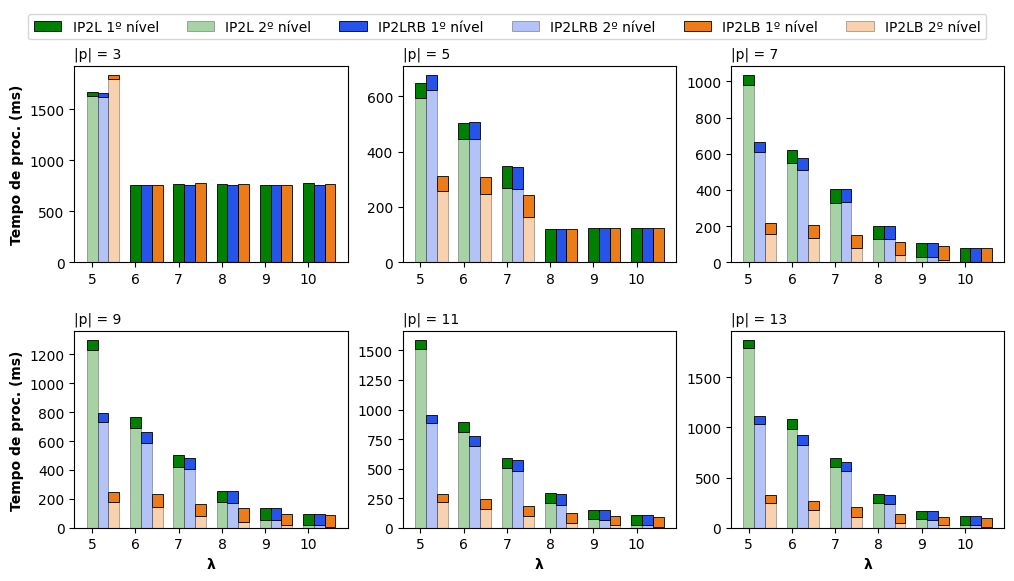
\includegraphics[width=1.0\textwidth]{figures/methods_processing_time_usaddr_3.png}
    \caption{Gráficos de barras empilhadas agrupadas por método (IP2L, IP2LB e IP2LRB) com o tempo de processamento (ms) em cada valor de $\lambda$ variando de $5$ a $10$, para $\tau=3$ e a base USADDR.}
    \label{fig:methods_processing_time_usaddr_3}
\end{figure}


% Please add the following required packages to your document preamble:
% \usepackage{graphicx}
\begin{table}[h]
\centering
\resizebox{\textwidth}{!}{%
\begin{tabular}{c|ccc|ccc|ccc|ccc|ccc|ccc|}
\cline{2-19}
\multicolumn{1}{l|}{} & \multicolumn{3}{c|}{$|p|=3$} & \multicolumn{3}{c|}{$|p|=5$} & \multicolumn{3}{c|}{$|p|=7$} & \multicolumn{3}{c|}{$|p|=9$} & \multicolumn{3}{c|}{$|p|=11$} & \multicolumn{3}{c|}{$|p|=13$} \\ \hline
\multicolumn{1}{|c|}{\textbf{Método}} & \multicolumn{1}{c|}{\textbf{1º}} & \multicolumn{1}{c|}{\textbf{2º}} & \textbf{total} & \multicolumn{1}{c|}{\textbf{1º}} & \multicolumn{1}{c|}{\textbf{2º}} & \textbf{total} & \multicolumn{1}{c|}{\textbf{1º}} & \multicolumn{1}{c|}{\textbf{2º}} & \textbf{total} & \multicolumn{1}{c|}{\textbf{1º}} & \multicolumn{1}{c|}{\textbf{2º}} & \textbf{total} & \multicolumn{1}{c|}{\textbf{1º}} & \multicolumn{1}{c|}{\textbf{2º}} & \textbf{total} & \multicolumn{1}{c|}{\textbf{1º}} & \multicolumn{1}{c|}{\textbf{2º}} & \textbf{total} \\ \hline
\multicolumn{1}{|c|}{IP2L-5} & 41,39 & 1625,46 & 1.666,86 & 53,27 & 593,77 & 647,05 & 56,90 & 977,63 & 1.034,54 & 63,45 & 1233,59 & 1.297,04 & 69,20 & 1514,61 & 1.583,81 & 74,64 & 1790,53 & 1.865,17 \\
\multicolumn{1}{|c|}{IP2LB-5} & 36,97 & 1795,61 & 1.832,59 & 53,68 & 256,66 & 310,34 & 61,36 & 157,97 & 219,33 & 65,11 & 179,83 & 244,94 & 69,46 & 215,19 & 284,65 & 75,59 & 246,6 & 322,20 \\
\multicolumn{1}{|c|}{IP2LRB-5} & 40,79 & 1614,34 & 1.655,14 & 53,94 & 622,48 & 676,42 & 57,86 & 609,44 & 667,30 & 64,44 & 729,97 & 794,41 & 71,53 & 885,04 & 956,57 & 75,67 & 1036,04 & 1.111,71 \\ \hline
\multicolumn{1}{|c|}{IP2L-6} & 757,67 &  & 757,67 & 58,56 & 445,29 & 503,85 & 71,06 & 550,25 & 621,31 & 77,33 & 688,58 & 765,90 & 84,22 & 812,75 & 896,98 & 97,82 & 983,63 & 1.081,45 \\
\multicolumn{1}{|c|}{IP2LB-6} & 753,98 &  & 753,98 & 60,19 & 246,68 & 306,87 & 72,04 & 134,18 & 206,22 & 91,43 & 144,78 & 236,21 & 83,84 & 160,45 & 244,29 & 90,18 & 180,22 & 270,40 \\
\multicolumn{1}{|c|}{IP2LRB-6} & 757,52 &  & 757,52 & 59,61 & 446,8 & 506,41 & 71,78 & 507,34 & 579,12 & 77,71 & 584,64 & 662,35 & 85,72 & 687,85 & 773,56 & 91,75 & 827,45 & 919,19 \\ \hline
\multicolumn{1}{|c|}{IP2L-7} & 762,05 &  & 762,05 & 77,60 & 268,94 & 346,54 & 78,44 & 327,75 & 406,19 & 80,88 & 420,2 & 501,08 & 87,99 & 502,22 & 590,21 & 92,55 & 602,49 & 695,04 \\
\multicolumn{1}{|c|}{IP2LB-7} & 776,22 &  & 776,22 & 79,32 & 163,18 & 242,50 & 72,95 & 76,95 & 149,90 & 81,90 & 82,62 & 164,52 & 90,41 & 95,85 & 186,26 & 95,57 & 108,26 & 203,82 \\
\multicolumn{1}{|c|}{IP2LRB-7} & 758,10 &  & 758,10 & 77,28 & 266,47 & 343,75 & 73,56 & 331,23 & 404,79 & 81,73 & 403,39 & 485,13 & 87,21 & 481,91 & 569,12 & 93,28 & 560,85 & 654,14 \\ \hline
\multicolumn{1}{|c|}{IP2L-8} & 763,83 &  & 763,83 & 119,97 &  & 119,97 & 71,12 & 129,78 & 200,90 & 80,09 & 177,22 & 257,31 & 84,63 & 206,1 & 290,73 & 88,22 & 245,58 & 333,80 \\
\multicolumn{1}{|c|}{IP2LB-8} & 767,97 &  & 767,97 & 120,75 &  & 120,75 & 71,36 & 39,17 & 110,53 & 95,76 & 38,54 & 134,30 & 86,43 & 41,6 & 128,03 & 90,55 & 49,52 & 140,06 \\
\multicolumn{1}{|c|}{IP2LRB-8} & 756,98 &  & 756,98 & 119,51 &  & 119,51 & 73,81 & 126,84 & 200,64 & 83,00 & 173,06 & 256,07 & 89,44 & 195,64 & 285,08 & 89,38 & 240,48 & 329,86 \\ \hline
\multicolumn{1}{|c|}{IP2L-9} & 761,45 &  & 761,45 & 124,54 &  & 124,54 & 73,61 & 31,91 & 105,52 & 80,44 & 55,04 & 135,48 & 83,15 & 70,06 & 153,21 & 86,41 & 83,45 & 169,85 \\
\multicolumn{1}{|c|}{IP2LB-9} & 761,63 &  & 761,63 & 124,65 &  & 124,65 & 74,05 & 14,17 & 88,21 & 79,34 & 17,14 & 96,48 & 83,38 & 18,81 & 102,20 & 88,58 & 22,19 & 110,76 \\
\multicolumn{1}{|c|}{IP2LRB-9} & 758,85 &  & 758,85 & 122,46 &  & 122,46 & 74,57 & 31,53 & 106,10 & 79,59 & 56,64 & 136,23 & 84,99 & 67,52 & 152,51 & 87,77 & 79,25 & 167,02 \\ \hline
\multicolumn{1}{|c|}{IP2L-10} & 777,05 &  & 777,05 & 124,02 &  & 124,02 & 77,19 &  & 77,19 & 79,20 & 15,92 & 95,12 & 84,51 & 22,43 & 106,94 & 87,83 & 29,22 & 117,05 \\
\multicolumn{1}{|c|}{IP2LB-10} & 762,56 &  & 762,56 & 123,70 &  & 123,70 & 77,57 &  & 77,57 & 78,73 & 7,7 & 86,43 & 82,84 & 7,84 & 90,67 & 87,37 & 9,88 & 97,25 \\
\multicolumn{1}{|c|}{IP2LRB-10} & 761,06 &  & 761,06 & 124,05 &  & 124,05 & 78,20 &  & 78,20 & 81,38 & 16,18 & 97,56 & 84,00 & 21,68 & 105,68 & 87,05 & 27,47 & 114,52 \\ \hline
\end{tabular}%
}
\caption{Tempo de processamento (ms) dos métodos IP2L, IP2LB e IP2LRB para prefixos de consulta com tamanho $3,5,6,9,11$ e $13$, valores de $\lambda$ variando de $5$ a $10$, e para $\tau=3$ na base de dados USADDR.}
\label{tab:methods-processing-time-tau-3-USADDR}
\end{table}

\newpage
\newpage
\subsection{Consumo de memória}
\label{sec:memory_consumption}

Os sistemas de CATE mantêm seus índices e os textos das sugestões armazenados diretamente na memória pois isso possibilita uma maior velocidade de acesso às informações e também responder às consultas por prefixos com mais velocidade. No entanto, é necessário equilibrar bem essa relação entre tempo de processamento e memória, pois ela é um recurso limitado e custoso. Nesse cenário, quanto maior o índice maior é a quantidade de memória utilizada. Por exemplo método IncNG\textit{Trie} \citep{xiao2013efficient}, apesar de ser o mais rápido presente na literatura, consome uma imensa quantidade de memória, o que dificulta utilizá-lo em alguns cenários práticos.

% Please add the following required packages to your document preamble:
% \usepackage{graphicx}
\begin{table}[]
\centering
\resizebox{0.60\textwidth}{!}{%
\begin{tabular}{c|c|c|c|}
\cline{2-4}
\multicolumn{1}{l|}{\textbf{}} & \textbf{AOL} & \textbf{USADDR} & \textbf{JUSBRASIL} \\ \hline
\multicolumn{1}{|c|}{\textbf{Método}} & \textbf{\begin{tabular}[c]{@{}c@{}}Memória \\ (MB)\end{tabular}} & \textbf{\begin{tabular}[c]{@{}c@{}}Memória \\ (MB)\end{tabular}} & \textbf{\begin{tabular}[c]{@{}c@{}}Memória \\ (MB)\end{tabular}} \\ \hline
\multicolumn{1}{|c|}{IP2L-5} & 37,99 & 1283,41 & 4757,45 \\
\multicolumn{1}{|c|}{IP2LRB-5} & 38,01 & 1282,76 & 4757,45 \\
\multicolumn{1}{|c|}{IP2LB-5} & 37,57 & 1253,34 & 4604,35 \\ \hline
\multicolumn{1}{|c|}{IP2L-6} & 45,22 & 1456,02 & 4733,27 \\
\multicolumn{1}{|c|}{IP2LRB-6} & 45,20 & 1455,46 & 4733,30 \\
\multicolumn{1}{|c|}{IP2LB-6} & 45,03 & 1446,06 & 4526,59 \\ \hline
\multicolumn{1}{|c|}{IP2L-7} & 55,92 & 1771,89 & 4680,71 \\
\multicolumn{1}{|c|}{IP2LRB-7} & 55,96 & 1771,86 & 4680,71 \\
\multicolumn{1}{|c|}{IP2LB-7} & 55,88 & 1770,87 & 4680,68 \\ \hline
\multicolumn{1}{|c|}{IP2L-8} & 69,22 & 2244,95 & 5018,19 \\
\multicolumn{1}{|c|}{IP2LRB-8} & 69,23 & 2244,90 & 5018,26 \\
\multicolumn{1}{|c|}{IP2LB-8} & 69,14 & 2243,90 & 5018,23 \\ \hline
\multicolumn{1}{|c|}{IP2L-9} & 84,22 & 2881,84 & 5604,38 \\
\multicolumn{1}{|c|}{IP2LRB-9} & 84,21 & 2881,87 & 5604,40 \\
\multicolumn{1}{|c|}{IP2LB-9} & 84,17 & 2881,72 & 5604,42 \\ \hline
\multicolumn{1}{|c|}{IP2L-10} & 100,67 & 3675,90 & 6496,82 \\
\multicolumn{1}{|c|}{IP2LRB-10} & 100,70 & 3675,88 & 6496,84 \\
\multicolumn{1}{|c|}{IP2LB-10} & 100,70 & 3675,87 & 6496,88 \\ \hline
\end{tabular}%
}
\caption{Quantidades de memória em \textit{MegaBytes} utilizadas pelos métodos IP2L, IP2LB, e IP2LRB, variando o parâmetro $\lambda$ de $5$ até $10$, para as bases AOL, USADDR, e JUSBRASIL.}
\label{tab:methods-memory-consumption}
\end{table}

A Tabela~\ref{tab:methods-memory-consumption} apresenta a quantidade média de memória (para todas as medições de memória para $\tau$ variando de $1$ a $3$ e $|p|$ variando de $3$ a $13$) em \textit{MegaBytes} de cada um dos três métodos propostos, com $\lambda$ variando de $5$ a $10$, para cada uma das bases AOL, USADDR, JUSBRASIL. A Figura~\ref{fig:memory_consumption_usaddr} contém um gráfico de barras que representa os dados da Tabela~\ref{tab:methods-memory-consumption} para o consumo de memória dos métodos para a base USADDR.

Podemos observar tanto na Tabela~\ref{tab:methods-memory-consumption} que a média de memória utilizada pelos três métodos é muito similar para cada valor de $\lambda$ experimentado, restando apenas a diferença de tempo de processamento para se comparar entre os métodos para um mesmo valor de $\lambda$. No entanto, as quantidades de memória diferem de forma relevante entre $\lambda=5$ e $\lambda=8$, ou $\lambda=6$ e $\lambda=10$, por exemplo. Na base USADDR o método IP2L-5 utilizou uma média de 1283,41 \textit{MegaBytes} de memória, enquanto o IP2L-8 utilizou 2244,95, quase $75\%$ a mais. Para a mesma base, o método IP2LB-6 utilizou 1446,06 enquanto o IP2LB-10 consumiu cerca de $250\%$ a mais com 3675,87. Nota-se que à medida em que $\lambda$ aumenta, cresce cada vez mais a diferença entre a quantidade de memória utilizada em relação ao valor anterior de $\lambda$. 

\begin{figure} [h]
    \centering
    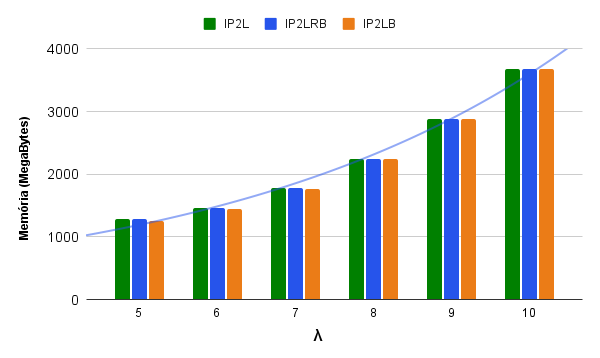
\includegraphics[width=0.80\textwidth]{figures/memory_usaddr.png}
    \caption{Gráfico de barras agrupadas por método (IP2L, IP2LB e IP2LRB) com a média de memória (\textit{MegaBytes}) utilizada para cada valor de $\lambda$ variando de $5$ a $10$, na base USADDR.}
    \label{fig:memory_consumption_usaddr}
\end{figure}

A Figura~\ref{fig:memory_consumption_usaddr} mostra o padrão de crescimento da média de memória utilizada para a base USADDR, por exemplo. A tendência de crescimento parece ser uma função exponencial crescente, representada na Figura~\ref{fig:memory_consumption_usaddr} pela linha azul que acompanha os grupos de barras. Quando não há muitos prefixos em comum nos itens indexados em uma \textit{Trie} ela pode acabar crescendo em um passo exponencial no tamanho do alfabeto $\Sigma$.  No entanto, vale ressaltar que a quantidade de memória utilizada pode estagnar em uma constante para um valores de $\lambda$ muito grandes. Se a maior sugestão de consulta de uma base possuir um tamanho de 20 caracteres, as quantidade de memória utilizadas para cada valor de $\lambda$ para $\lambda \geq 20$ serão iguais. Feita a ressalva, podemos analisar o gráfico ``localmente'' para $\lambda \leq 10$.

A linha de tendência apresentada na Figura~\ref{fig:memory_consumption_usaddr} é uma representação da função $f(\lambda)=1190\cdot e^{0,22\cdot\lambda}$. Ora, esse é um formato de função (exponencial crescente) similar às funções de tendência de tempo de processamento (exponencial decrescente) apresentadas na seção~\ref{sec:methods-processing-time}. Quando há poucos nós na \textit{Trie} utilizada no primeiro nível o tempo de processamento é bem alto, mas à medida em que $\lambda$ aumenta, também há um crescimento com tendência exponencial no número total de nós dessa \textit{Trie} que por consequência aumenta a quantidade de informação disponível para a busca tolerante a erros, reduzindo o tempo de processamento. Essa é uma forte evidência da relação entre a memória e desempenho de um método de CATE, principalmente nos métodos que seguem a abordagem em dois níveis.

Para a base JUSBRASIL ocorreu uma peculiaridade nas quantidades de memória: entre $\lambda=5$ e $\lambda=7$ a memória utilizada vai diminuindo em um passo lento, e só a a partir de $\lambda=8$ começa a aumentar, com um passo mais rápido Isso acontece provavelmente devido à natureza da base, a qual foi extraída de \textit{logs} de um sistema real de CATE. É mais frequente a quantidade de prefixos em comum entre os primeiros caracteres das sugestões de consulta. A partir de $\lambda=8$ os prefixos já começam a ficar mais difusos, e a Trie começa a crescer bastante em largura, aumentando quantidade de nós necessários para indexá-los.

O contexto e cenário de um sistema de CATE podem influenciar a escolha do valor ideal para $\lambda$. Deve-se levar em conta o tamanho médio dos prefixos de consulta que se espera receber no sistema, o número de sugestões na base para se indexar, o tamanho médio dessas sugestões, e a quantidade de memória disponível. 

Por fim, selecionamos os modelos IP2L-10, IP2LRB-10 e IP2LB-10 para serem comparados com os métodos de base na seção~\ref{sec:comparison_baseline_methods} a seguir. Dentre os valores de $\lambda$ e $\tau$ experimentados o valor $\lambda=10$ foi o que mais aproximou o tempo de processamento dos métodos do limite de $100ms$ para bases grandes como USADDR e JUSBRASIL. Além disso, mesmo para $\lambda=10$ a economia de memória em relação ao método ICPAN original chega a ser mais de $50\%$ como será demonstrado na próxima seção.


\section{Comparação com os Métodos de Base}
\label{sec:comparison_baseline_methods}

Nesta seção iremos comparar os métodos IP2L-10, IP2LB-10 e IP2LRB-10 com os métodos ICAN, ICPAN, e META (cujos códigos foram providos pelos autores) e também o método BEVA (implementação própria) nas bases AOL e USADDR. Analisaremos as médias de tempo de processamento em dois cenários: (1) variando o limiar $\tau$ de distância de edição para um prefixo de consulta mais curto de tamanho 5, e também mais longo, de tamanho 13; (2) média de tempos de processamento para $\tau=3$, variando o tamanho do prefixo de 3 a 13, de 2 em 2. Por fim, analisaremos também a utilização de memoria.

\subsection{Variando o valor do Limiar de Distância de Edição}

As Tabelas \ref{tab:baselines-varying-tau-p-5} e \ref{tab:baselines-varying-tau-p-13} contêm os tempos de processamento para todos os algoritmos variando $\tau$ de 1 a 3, e com os tamanhos de prefixo de consulta fixados em 5 e 13, respectivamente, com o objetivo de analisar o resultados para tamanhos de prefixos de consulta mais pequenos e mais longos. Nesse último cenário o segundo nível pode vir a ter um mal desempenho quando precisa buscar por cadeias de caracteres muito longas, principalmente o IP2L que realiza apenas busca sequencial. Quanto maior é o tamanho da cadeia de caracteres buscada no segundo nível, maior é o tempo de execução do cálculo da matriz de \textit{Levenhstein}. Já que $\lambda$ está fixado em 10, para o tamanho $|p|=13$ o segundo nível é sempre ativado para os valores de $\tau$ experimentados.

\begin{table}[h]
\centering
\begin{tabular}{c|c|c|c|c|c|c|}
\cline{2-7}
\multicolumn{1}{l|}{} & \multicolumn{3}{c|}{\textbf{AOL}} & \multicolumn{3}{c|}{\textbf{USADDR}} \\ \hline
\multicolumn{1}{|c|}{\textbf{Método}} & $\tau=1$ & $\tau=2$ & $\tau=3$ & $\tau=1$ & $\tau=2$ & $\tau=3$ \\ \hline
\multicolumn{1}{|c|}{IP2L-10} & 0,15 & 0,80 & 3,23 & 0,70 & 9,24 & 124,02 \\ \hline
\multicolumn{1}{|c|}{IP2LB-10} & 0,15 & 0,81 & 3,22 & 0,70 & 9,31 & 123,70 \\ \hline
\multicolumn{1}{|c|}{IP2LRB-10} & 0,16 & 0,86 & 3,56 & 0,72 & 9,26 & 124,05 \\ \hline
\multicolumn{1}{|c|}{ICAN} & 0,09 & 1,59 & 10,97 & 0,30 & 8,14 & 165,98 \\ \hline
\multicolumn{1}{|c|}{ICPAN} & 0,17 & 1,05 & 4,22 & 0,73 & 10,79 & 154,05 \\ \hline
\multicolumn{1}{|c|}{BEVA} & 0,25 & 1,42 & 3,92 & 0,72 & 9,31 & 51,85 \\ \hline
\multicolumn{1}{|c|}{META} & 0,07 & 1,46 & 25,88 & 0,33 & 52,31 & 4572,78 \\ \hline
\end{tabular}
\caption{Tempos de processamento dos algoritmos em dois níveis propostos com $\lambda=10$ e os outros métodos de base, para as bases de sugestões de consulta AOL e USADDR e $|p|=5$, com $\tau$ variando de $1$ a $3$.}
\label{tab:baselines-varying-tau-p-5}
\end{table}

Na base AOL, podemos observar na Tabela~\ref{tab:baselines-varying-tau-p-5} para $\tau=1$ que os tempos entre os métodos de dois níveis foram muito similares. O método ICAN desempenhou melhor do que todos com exceção do META, que foi o mais rápido. É importante ressaltar que, para $\lambda=10$ e $|p|=5$, apenas o primeiro nível é ativado para todos os valores de $\tau$ experimentados. 

Um claro efeito desse fato é que para $\tau=2$, por exemplo, podemos notar que os algoritmos de dois níveis propostos obtiveram tempo de processamento menores do que o ICPAN. Isso ocorre porque como a altura máxima da árvore é limitada no valor de $\lambda$, há muito menos nós para verificar e ativar do que no método ICPAN, que indexa as sugestões por completo no índice \textit{Trie}. Outro efeito é que os tempos entre os três métodos são bastante similares. Podemos notar esses dois padrões ocorrendo para todos os valores de $\tau$ nas bases AOL e USADDR. Para $\tau=2$ o método ICAN deixou de ser um dos mais rápidos, para se tornar o mais lento. Os métodos de dois níveis agora atingiram os menores tempos, o que é plausível pois como mencionado anteriormente, o primeiro nível desses métodos possuem um conjunto muito menor de nós para processar quando comparado aos métodos ICAN e ICPAN. 

Para $\tau=3$ os métodos de dois níveis seguem novamente com os menores tempos. Também é possível observar que os métodos ICAN e META sofreram grande aumento de tempo de processamento ao tolerar mais erros na busca. Em uma base pequena como a AOL verificamos que os métodos em dois níveis foram mais rápidos do que o BEVA, atualmente o método estado-da-arte.

Na base USADDR vemos novamente para $\tau=1$ que os métodos ICAN e META obtiveram os menores tempos. Tais métodos se demonstraram eficientes ao tolerar apenas um erro de digitação. O ICPAN e BEVA, e todos os métodos de dois níveis obtiveram tempos bem próximos. Para $\tau=2$ o método BEVA obteve um tempo próximo ao dos métodos de dois níveis. Diferentemente da base AOL, em uma base maior como a USADDR identificamos que o método BEVA obteve um desempenho bem próximo aos algoritmos de dois níveis, no entanto, demonstrou-se muito mais eficiente do que todos os outros métodos para $\tau=3$ com um tempo de 51,85\textit{ms}, sendo o único a atingir um tempo de processamento menor do que $100ms$. 

\begin{table}[h]
\centering
\begin{tabular}{c|c|c|c|c|c|c|}
\cline{2-7}
 & \multicolumn{3}{c|}{\textbf{AOL}} & \multicolumn{3}{c|}{\textbf{USADDR}} \\ \hline
\multicolumn{1}{|c|}{\textbf{Método}} & $\tau=1$ & $\tau=2$ & $\tau=3$ & $\tau=1$ & $\tau=2$ & $\tau=3$ \\ \hline
\multicolumn{1}{|c|}{IP2L-10} & 0,10 & 0,92 & 5,55 & 0,64 & 8,12 & 117,05 \\ \hline
\multicolumn{1}{|c|}{IP2LB-10} & 0,07 & 0,72 & 3,74 & 0,31 & 6,28 & 97,25 \\ \hline
\multicolumn{1}{|c|}{IP2LRB-10} & 0,10 & 0,90 & 5,45 & 0,41 & 7,64 & 114,52 \\ \hline
\multicolumn{1}{|c|}{ICAN} & 0,11 & 1,90 & 13,89 & 0,34 & 10,20 & 215,06 \\ \hline
\multicolumn{1}{|c|}{ICPAN} & 0,10 & 1,02 & 4,75 & 0,35 & 8,07 & 130,38 \\ \hline
\multicolumn{1}{|c|}{BEVA} & 0,33 & 1,80 & 5,49 & 0,92 & 12,13 & 78,85 \\ \hline
\multicolumn{1}{|c|}{META} & 0,20 & 2,95 & 38,81 & 0,80 & 74,64 & 6006,38 \\ \hline
\end{tabular}
\caption{Tempos de processamento dos algoritmos em dois níveis propostos com $\lambda=10$ e os outros métodos de base, para as bases de sugestões de consulta AOL e USADDR e $|p|=13$, com $\tau$ variando de $1$ a $3$.}
\label{tab:baselines-varying-tau-p-13}
\end{table}

Na Tabela~\ref{tab:baselines-varying-tau-p-13} para a base AOL podemos observar que quando $\tau=1$ há uma diferença sutil entre o tempo do IP2LB-10 e os tempos dos outros dois métodos de dois níveis. Com $|p|=13$ o segundo nível está sendo ativado, então as diferenças de eficiência do segundo nível começam a aparecer. O IP2LB-10 foi o que obteve o menor tempo de processamento. Vale ressaltar no entanto que a acurácia é baixa para $\tau=1$ e relativamente baixa para $\tau=2$, como foi demonstrado na seção~\ref{sec:binary-search-impact-on-two-level}. O tempo do ICPAN foi bem similar aos do IP2L-10 e IP2LRB-10. Para $\tau=2$ pode-se notar que os tempos dos métodos IP2L-10 e IP2LRB-10 foram um pouco menores do que o ICPAN. A diferença entre o tempo do IP2LB-10 e os outros dois métodos de dois níveis já aparenta ser um pouco mais expressiva. Os algoritmos de dois níveis obtiveram os menores tempos de processamento. Para $\tau=3$ o bom desempenho do IP2LB-10 pode ser notado com mais clareza pois atingiu um tempo de 3,74\textit{ms} (menor tempo dentre os algoritmos), sendo aproximadamente 1,5 vezes mais rápido do que o IP2L-10, que obteve um tempo de 5,55\textit{ms}. O IP2L-10 foi o único método em dois níveis que teve um tempo de processamento maior do que o BEVA para $\tau=3$. Além disso, os tempos do IP2L-10 e IP2LRB-10 agora foram maiores do que o ICPAN.

Na base USADDR e $\tau=1$, o método IP2L-10 obteve um tempo quase 2 vezes mais lento do que o ICPAN, no entanto, ainda com um tempo eficiente de menos de 1\textit{ms}. Além disso, todos os métodos de base também obtiveram tempo menor que 1\textit{ms}. O IP2LB-10 obteve o menor tempo para $\tau=1$ e $\tau=2$, no entanto, possui os problemas de acurácia nesses casos mencionados na seção~\ref{sec:binary-search-impact-on-two-level}. Para $\tau=2$, o IP2LRB-10 ficou logo atrás do IP2L-10, obtendo o segundo menor tempo. Também podemos verificar que o desempenho de 8,12\textit{ms} do IP2L-10 se aproximou mais do ICPAN, com 8,07\textit{ms}, ou seja, uma diferença de apenas 0,05\textit{ms}. Para $\tau=3$, em uma base grande como a USADDR a dificuldade do desafio de CATE se torna mais nítida, bem como a eficiência do método BEVA, que foi o único a conseguir um tempo de processamento menor do que 100\textit{ms} sem ter problemas de acurácia, e ainda com uma boa margem em relação aos outros métodos. No entanto, vale destacar que o método IP2LB-10 também obteve tempo menor do que 100\textit{ms}, e como $\tau=3$, sua acurácia é mais passível de se utilizar em um sistema real de CATE. 

Outra situação ocorrida é que o IP2L-10 obteve 117,05\textit{ms} um tempo de processamento menor do que o ICPAN, com 130,38\textit{ms}. E preciso considerar que o IP2L-10 realiza uma busca tolerante a erros no primeiro nível em uma árvore de altura profundidade máxima igual a 10, e então buscar sequencialmente no segundo nível por $p$. Além disso, para valores maiores de $\lambda$, frequentemente o tamanho das listas em que se realiza a busca sequencial e menor quando o segundo nível é ativado. Uma vez que $|p|=13$ e $\tau=3$, o ICPAN precisa realizar a busca tolerante a erros em uma profundidade máxima de $|p| + \tau = 16$ caracteres para responder ao prefixo de consulta $p$. Diferentemente do que ocorreu na base AOL para $\tau=3$, o experimento indica que possivelmente em uma base grande como o USADDR e com uma tolerância maior a erros como $\tau=3$, o processamento de nós com uma maior profundidade na árvore do ICPAN é mais lento do que combinar o processamento desses nós em uma profundidade menor com busca sequencial.


\subsection{Variando o Tamanho do Prefixo de Consulta}

As Tabelas \ref{tab:baselines-varying-prefix-size-AOL} e \ref{tab:baselines-varying-prefix-size-USADDR} contêm os tempos de processamento médios para todos os algoritmos com o tamanho do prefixo de consulta variando de $|p|=3$ até $|p|=13$ de 2 em 2 com $\tau=3$ para as bases AOL e USADDR, respectivamente. Consideramos apenas $\tau=3$ seguindo a literatura, pois isso nos permite analisar o processamento das consultas dos métodos com um número relevante de erros de digitação. Valores acima de 3 não são comuns em cenários práticos de CATE.

\begin{table}[h]
\centering
\begin{tabular}{c|c|c|c|c|c|c|}
\cline{2-7}
\multicolumn{1}{l|}{} & \multicolumn{6}{c|}{\textbf{AOL}} \\ \hline
\multicolumn{1}{|c|}{\textbf{Método}} & $|p| =  3$ & $|p| =  5$ & $|p| =  7$ & $|p| =  9$ & $|p| =  11$ & $|p| =  13$ \\ \hline
\multicolumn{1}{|c|}{IP2L-10} & 11,81 & 3,23 & 2,77 & 4,10 & 5,15 & 5,55 \\ \hline
\multicolumn{1}{|c|}{IP2LB-10} & 11,86 & 3,22 & 2,77 & 3,43 & 3,73 & 3,74 \\ \hline
\multicolumn{1}{|c|}{IP2LRB-10} & 11,85 & 3,56 & 2,94 & 4,55 & 5,70 & 5,45 \\ \hline
\multicolumn{1}{|c|}{ICAN} & 14,31 & 10,97 & 12,40 & 12,99 & 13,93 & 13,89 \\ \hline
\multicolumn{1}{|c|}{ICPAN} & 11,21 & 4,22 & 4,17 & 4,41 & 4,70 & 4,75 \\ \hline
\multicolumn{1}{|c|}{BEVA} & 0,004 & 3,92 & 4,90 & 5,22 & 5,45 & 5,49 \\ \hline
\multicolumn{1}{|c|}{META} & 11,27 & 25,88 & 31,77 & 34,76 & 37,57 & 38,81 \\ \hline
\end{tabular}
\caption{Tempos de processamento médios dos métodos propostos com $\lambda=10$ e dos métodos de base para $\tau=3$, na base de sugestões de consultas AOL, variando o tamanho do prefixo de consulta de 3 a 13, de 2 em 2.}
\label{tab:baselines-varying-prefix-size-AOL}
\end{table}

Na Tabela~\ref{tab:baselines-varying-prefix-size-AOL} podemos observar que o método BEVA obteve um tempo de processamento muito baixo de 0,004\textit{ms} para um tamanho pequeno de prefixo de consulta como $|p|=3$. Esse fato também se repetiu para a base USADDR, como podemos ver na Tabela~\ref{tab:baselines-varying-prefix-size-USADDR}. Isso ocorre porque a implementação do BEVA utilizada neste trabalho implementa uma política de \textit{cache} de nós ativos para reduzir o tempo de processamento para prefixos de consulta muito curtos. Uma característica que os métodos em dois níveis, o ICAN, ICPAN, BEVA e META possuem em comum é que para valores maiores de $\tau$ e prefixos muito curtos há uma quantidade massiva de nós da \textit{Trie} para ativar/visitar. Os autores do IncNG\textit{Trie} \citep{xiao2013efficient} e IncNG\textit{Trie}+ \citep{qin2020efficient} denominam esse problema como ``explosão da fase inicial''. O restante dos métodos obtiveram tempos de processamento próximos, com exceção do ICAN, que foi o mais lento com 14,31\textit{ms}. Com $|p|=5$ a política de \textit{cache} do BEVA já não é mais ativada, e seus tempos entram em uma faixa mais próxima dos outros métodos; os métodos de dois níveis atingiram os menores tempos de processamento, e assim permanece até $|p|=9$. No entanto, seguem obtendo tempos competitivos com o ICPAN e BEVA para $|p|=11$ e $|p|=13$. Também vale destacar que o método IP2LB-10 seguiu com os menores tempos de processamento a partir de $|p|=5$ até $|p|=13$.

\begin{table}[h]
\centering
\begin{tabular}{c|c|c|c|c|c|c|}
\cline{2-7}
\multicolumn{1}{l|}{} & \multicolumn{6}{c|}{\textbf{USADDR}} \\ \hline
\multicolumn{1}{|c|}{\textbf{Método}} & $|p| =  3$ & $|p| =  5$ & $|p| =  7$ & $|p| =  9$ & $|p| =  11$ & $|p| =  13$ \\ \hline
\multicolumn{1}{|c|}{IP2L-10} & 777,05 & 124,02 & 77,19 & 95,12 & 106,94 & 117,05 \\ \hline
\multicolumn{1}{|c|}{IP2LB-10} & 762,56 & 123,70 & 77,57 & 86,43 & 90,67 & 97,25 \\ \hline
\multicolumn{1}{|c|}{IP2LRB-10} & 761,06 & 124,05 & 78,20 & 97,56 & 105,68 & 114,52 \\ \hline
\multicolumn{1}{|c|}{ICAN} & 381,29 & 165,98 & 171,89 & 217,98 & 208,36 & 215,06 \\ \hline
\multicolumn{1}{|c|}{ICPAN} & 759,18 & 154,05 & 110,71 & 115,35 & 124,94 & 130,38 \\ \hline
\multicolumn{1}{|c|}{BEVA} & 0,01 & 51,85 & 68,33 & 75,49 & 77,23 & 78,85 \\ \hline
\multicolumn{1}{|c|}{META} & 2400,16 & 4572,78 & 5140,76 & 5656,81 & 5864,68 & 6006,38 \\ \hline
\end{tabular}
\caption{Tempos de processamento médios dos métodos propostos com $\lambda=10$ e dos métodos de base para $\tau=3$, na base de sugestões de consultas USADDR, variando o tamanho do prefixo de consulta de 3 a 13, de 2 em 2.}
\label{tab:baselines-varying-prefix-size-USADDR}
\end{table}

Na Tabela~\ref{tab:baselines-varying-prefix-size-AOL} para $|p|=3$ vemos novamente o impacto da política de \textit{cache} do BEVA, que respondeu as consultas com uma média de 0,01\textit{ms} apenas. Os métodos de dois níveis, o META e o ICPAN obtiveram tempo maior do que 700\textit{ms} para responder às consultas, e com certeza também se beneficiariam de uma política de \textit{cache} como a do BEVA. O META seguiu com os maiores tempos em todos os tamanhos de $p$. Além disso, nem o ICAN ou o ICPAN conseguiram obter uma média de tempo menor do que 100\textit{ms} em qualquer valor de $|p|$. 

Diferentemente da base AOL, a eficiência do método BEVA fica mais clara em uma base maior como a USADDR. O método BEVA obteve os menores tempos para todos os tamanhos de $|p|$ como podemos observar na Tabela~\ref{tab:baselines-varying-prefix-size-USADDR}. Para $|p|=7$ e $|p|=9$ os métodos de dois níveis foram os únicos além do BEVA a atingir tempos menores do que 100\textit{ms}. O método IP2L-10 por exemplo obteve 77,18\textit{ms} para $|p|=7$, sendo cerca de 1,4 vezes mais rápido do que o ICPAN com 110,71\textit{ms}. No entanto, a partir de $|p|=11$ os métodos IP2L-10 e IP2LRB-10 seguem com tempos maiores do que 100\textit{ms}. É necessário destacar o desempenho do IP2LB-10, que obteve tempos abaixo de 100\textit{ms} para todos os tamanhos de prefixo de consulta a partir de $|p|=7$. Além disso, o método IP2L-10 (que não tem problemas com acurácia) demonstrou médias de tempo menores do que o ICPAN para todos os tamanhos de prefixo de consulta a partir de $|p|=5$, algo que no cenário experimentado pode indicar que a solução em dois níveis se demonstrou mais vantajosa do que o método original utilizado no primeiro nível no quesito tempo de processamento.

\subsection{Consumo de memória}

Quando comparamos o consumo de memória, notamos que os métodos propostos apresentam uma vantagem em comparação aos métodos de base. A Tabela~\ref{tab:baselines-memory-consumption} apresenta a quantidade média de memória utilizada pelos métodos propostos e os de base para os 3 valores de $\tau$ experimentados (cada célula contém a média aritmética entre as quantidades de memória medidas para $\tau=1$, $\tau=2$ e $\tau=3$), nas bases AOL, USADDR e JUSBRASIL. Para todas as bases podemos observar que os métodos propostos obtiveram o menor consumo de memória. 

\begin{table}[h]
\centering
\begin{tabular}{c|c|c|c|}
\cline{2-4}
\multicolumn{1}{l|}{} & \textbf{AOL} & \textbf{USADDR} & \textbf{JUSBRASIL} \\ \hline
\multicolumn{1}{|c|}{\textbf{Método}} & \textbf{Memória (MB)} & \textbf{Memória (MB)} & \textbf{Memória (MB)} \\ \hline
\multicolumn{1}{|c|}{IP2L-10} & 107,11 & 4070,68 & 6747,79 \\ \hline
\multicolumn{1}{|c|}{IP2LB-10} & 107,25 & 4070,73 & 6747,86 \\ \hline
\multicolumn{1}{|c|}{IP2LRB-10} & 107,19 & 4070,71 & 6747,76 \\ \hline
\multicolumn{1}{|c|}{ICAN} & 603,76 & 10833,27 & - \\ \hline
\multicolumn{1}{|c|}{ICPAN} & 362,59 & 9807,05 & - \\ \hline
\multicolumn{1}{|c|}{BEVA} & 215,91 & 5962,14 & 19232,93 \\ \hline
\multicolumn{1}{|c|}{META} & 262,31 & 7481,40 & - \\ \hline
\end{tabular}
\caption{Quantidades médias de memória em \textit{MegaBytes} utilizadas pelos métodos de base e métodos IP2L, IP2LB, e IP2LRB durante o processamento das consultas para os 3 valores de $\tau$ experimentados, com o parâmetro $\lambda=10$ para as bases AOL, USADDR, e JUSBRASIL.}
\label{tab:baselines-memory-consumption}
\end{table}

Na base AOL, os algoritmos de dois níveis economizaram cerca de $82\%$ de memória em relação ao ICAN, $70\%$ em relação ao ICPAN, e $50\%$ em relação ao BEVA. Além disso, vale comentar que o ICAN foi o método com os maiores consumos de memória. Isso ocorre provavelmente porque, devido ao funcionamento do algoritmo ICAN quanto à manutenção dos conjuntos de nós ativos para o processamento da consulta, o tamanho desses conjuntos pode ser demasiadamente grande. Isso causa uma adição à quantidade de memória já utilizada para o índice. Para ilustrar essa adição basta comparar o método ICAN com o ICPAN. Os dois possuem índices com o mesmo tamanho, mas diferem bastante quanto ao tamanho dos conjuntos de nós ativos (diferença entre as cardinalidades $|\Phi_{p}|$ e $|\Psi_{p}|$, respectivamente). Na base USADDR o método ICPAN utilizou cerca de 9,57GB de memória e o BEVA utilizou 5,82GB, enquanto os métodos de dois níveis utilizaram cerca de 4GB, apresentando uma economia de $58\%$ e $31\%$, respectivamente. 

Na base JUSBRASIL, podemos observar uma economia ainda mais significativa em comparação com o BEVA. Os algoritmos de dois níveis economizaram cerca de quase $65\%$, pois utilizaram 6,58GB indexando os $\lambda=10$ primeiros caracteres das sugestões de consulta, enquanto o BEVA utilizou 18,78GB indexando o texto completo de cada item da base. Ainda há espaço para experimentar aumentar o valor de $\lambda$ de forma que o IP2LB-$\lambda$ provavelmente atinja tempos menores que 100\textit{ms} para $\tau=3$ e se torne utilizável para a base JUSBRASIL, enquanto garante uma boa economia de memoria em relação ao método BEVA. 

Diante dos resultados dos experimentos concluímos que a abordagem em dois níveis no contexto do problema de CATE provou-se efetiva. Além disso, também verificamos que a utilização da busca binária no segundo nível tanto nos métodos IP2LB quanto IP2LRB pode deixar a desejar quanto à acurácia para $\tau=1$ e $\tau=2$, mas pode atingir uma acurácia melhor para $\tau=3$, o qual é o limiar de tolerância que ocasionou os maiores tempos de processamento nos métodos de CATE nos experimentos. O método IP2LB apresenta uma redução significativa do tempo total de processamento em comparação com o IP2L para $\tau=3$, ultrapassando também o ICAN e ICPAN em todos os casos nas duas bases experimentadas, com exceção de $|p|=3$. O IP2L se demonstrou efetivo pois também teve um melhor desempenho do que o ICPAN em quase todos os casos, e assim como o IP2LB e IP2LRB também utilizou menores quantidades de memória.